\chapter{
%Basic Statistical Concepts
%Basic Statistical Concepts and Statistical Description of SCR Models
%Basic Statistical Concepts and the Hierarchy of SCR Models
Hierarchical Modeling and SCR
}
\markboth{Modeling}{}
\label{chapt.modeling}


\vspace{.3in}

In the previous chapter we described the basics of capture-recapture
methods and the advantages that spatial models have over
traditional non-spatial models. In doing so, we avoided statistical
terminology. Although it is critical to
understand the non-technical motivation for this broad class of
models, it is impossible to fully appreciate them, and apply them to
real data, without a solid grasp of the fundamentals of statistical
inference.

In this chapter, we present a brief overview of the key
statistical concepts that are referenced throughout the remainder of
this book. Emphasis is placed on the definition of a random variable,
the common probability distributions used to model random variables,
and how hierarchical models can be used to describe conditionally
related random variables. For some readers, this material will be
familiar, perhaps even elementary, and thus you may want to skip to the next
chapter. However, our experience is that many basic statistics courses
taken by ecologists do not emphasize the important subjects covered in
this chapter. Instead, there seems to be much attention paid to pedantics
such as
computing the number of degrees of freedom in
various $F$-tests which, although useful in some contexts, do not
provide the basis for drawing conclusions from data and evaluating
scientific hypotheses. %---the objectives of statistical inference.

The material in the
beginning of this chapter is explained in numerous other
texts. %\citet{casella_burger:2002}
Technical treatments that emphasize ecological
problems are given by
\citet{williams_etal:2002}, \citet{royle_dorazio:2008} and
\citet{link_barker:2010}, to name just a few. A very accessible introduction to some of the
topics covered in this chapter is presented in Chapt. 3 of
\citet{mackenzie_etal:2006}. With all these sources, one
might wonder why we bother rehashing these concepts here. Our motivation is
two-fold: first, we wish to develop this material using examples
relevant to spatial capture-recapture, and second, we find that most
introductory texts are not accompanied by code that can
be helpful to the novice. We therefore attempt to present simple \R~code
throughout this chapter so that those who struggle with equations and
mathematical notation can learn by doing. As mentioned in the Preface,
we rely on \R~because it provides tremendous flexibility for analyzing
data and because it is free. We do not, however, try to explain how to
use \R~because there are so many good references already, including
\citet{venables_ripley:2002,bolker:2008,venables_etal:2012}.

After covering some basic concepts of hierarchical modeling, we end the
chapter by describing spatial capture-recapture models using
hierarchical modeling notation. This makes the concepts outlined in
the previous chapter more precise, and it provides the basis for describing
variations on the basic them of combining models of the ecological
process of interest with models describing how the observations are
thought to arise conditional on the actual state of the system.

% Following our introduction to basic statistical concepts, we lay out our
% philosophy of modeling ecological data, including spatial
% capture-recapture data. We also introduce hierarchical
% models, and discuss why they are relevant to so many problems in
% ecology. Finally, we address the common concerns levied against the
% hierarchical modeler, {e.g.} assumptions are bad.

\section{Random Variables and Probability Distributions}

\subsection{Stochasticity in ecology}

%{\bf XXXXX We need to talk about use of X vs use of x. The usage here
%  is correct but we don't do this throughout the book XXXXX}

Few ecological processes can be described using purely deterministic
models, and thus we need a formal method for drawing conclusions from data while
acknowledging the stochastic nature of ecological systems and their observation. This is the role of statistical inference,
which is founded on the laws of probability. For our purposes, it
suffices to be familiar with a small number of concepts from
probability theory. The most important of which is the concept of a random
variable, say $X$. We wish to know the probability that a realization
of $X$ takes on some value $x$, %. That is, we want to be able to describe
$\text{Pr}(X=x)$, or perhaps the probability that $x$ lies within some
range of values. An approach for achieving such goals is to develop a
statistical model for $X$ and then estimate the parameters of the
model by fitting it to data collected during an experiment.

To clarify the concept of a random variable, let $X$ be the number of
American shad (\emph{Alosa sapidissima}) caught after $K=20$ casts at
the shad hole on Deerfield River in Massachusetts. Suppose that
we had a good day and caught $x=7$ fish. If there were no random
variation at play, we would say that the probability of catching a
fish, denoted $p$, is $p=7/20=0.35$, and therefore might think we would always catch 7 shad after 20
casts. In other words, our deterministic model is $x =
0.35\times K$. In reality, however, we can be pretty sure that this
deterministic model would not be very good. Even if we knew for
certain $p \equiv 0.35$, we would expect some variation in the number
of fish caught on repeated fishing outings. To describe this
variation, we need a model that acknowledges uncertainty (i.e.,
stochasticity), and specifically we need a model that describes the
probability of catching $x$ fish given $K$ and $p$,
$\text{Pr}(X=x|K,p)$.

To specify a model for $\text{Pr}(X=x|K,p)$ we need a specific type of
function known as a probability mass function (pmf). Or, in the case
where $X$ is a continuous random variable, we need a probability
density function (pdf). We will generically refer to these as
probability distributions.
Statisticians make things easier for themselves,
and more complicated for everyone else, by using different notation
for probability distributions. Sometimes you will see
$\text{Pr}(X=x|K,p)$ expressed as $f(X|K,p)$ or $f(X; K,p)$ or
$p(X|K,p)$ or $\pi(X|K,p)$ or $\mathbb{P}(X|K,p)$ or $[X|K,p]$ or even
just $[X]$! Just remember that these expressions all have the same
meaning---they are all probability distributions that tell us the
probability of observing any possible realization of the random
variable $X$.

In this book, we will almost always use bracket notation (the last two
examples above) to represent arbitrary probability distributions.
Hence, from here on out, when you see $[X|K,p]$, just remember that
this is equivalent to the more traditional (but perhaps less popular)
expression $\text{Pr}(X=x|K,p)$. Note that this probability distribution
could be virtually anything: Poisson, Gaussian, beta, etc $\dots$
In addition,
from here on, to achieve a more concise presentation, we will no longer use uppercase letters to denote
random variables and lowercase letters for realized values. Rather, we
will define a random variable by some symbol ($x$, $N$, $\theta$,
etc..) and let the context determine whether we are talking about the
random variable itself, or realized values of it.
%One reason
%for this is that we find it more convenient to let $N$ represent
%population size and $n$ represent a count statistic,
In some, limited, cases, we will want upper-
and lower-case letters to represent different variables. For example,
$N$ (population size)  and $n$ (sample size) is a typical example.
%We favor $[X|K,p]$ over
%$\text{Pr}(X=x|K,p)$ simply because the former is more concise and
%because we do not think it adds clarity to distingare that the former is more concise and is
%Hence, we will

When
we wish to be specific about a probability distribution, we will do
so in one of two ways, one mathematically precise and one symbolic. Before explaining
these two options, let's choose a specific distribution as a model for
the data in our example. In this case, the natural choice for
$[x|K,p]$ is the binomial distribution, the mathematically precise representation of
which is
%this distribution will be shown as:
\begin{equation}
  [x|K,p] = %\text{Bin}(K,p) =
             \binom{x}{K}p^x(1-p)^{K-x}.
  \label{modeling.eq.bin}
\end{equation}
The right-hand side of this equation is the binomial pmf (described in
more detail in Sec.~\ref{sec.modeling.distributions}), and plugging in
values for the parameters $K$, and $p$ will return the probability of
observing any realized value of the random variable $x$. This is precise, but it is also
cumbersome to write repetitively, and it may make the eyes glaze over
when seen too often. Thus, we will
often simplify Eq.~\ref{modeling.eq.bin} using the symbolic notation:
%{\bf XXXXX below -- little x or big X?? XXXXX}
\begin{equation}
  x \sim \text{Binomial}(K, p)
  \label{modeling.eq.binsym}
\end{equation}
%In cases where $x$ is continuous, we refer to
%$[x]$ as a probability density functions (pdf), or when
%$x$ is discrete, we call $[x]$ a probability mass functions (pmf).
%In parametric inference, we assume a particular distribution for $x$, which in
%this case would naturally be the binomial distribution, $x \sim
%\text{Binomial}(K, p)$, where $p$ is the
%probability of catching a shad on a particular cast and $K$ is the
%binomial size parameter.
The ``$\sim$'' symbol is meant to represent a stochastic relationship, and
can be read ``is distributed as.''
%We  will use this notation to complement the bracket notation, which will
%be reserved for generic probability distributions. Thus, we could
%refer to the distribution of $x$ as
%$[x]$, with possible options being $x \sim \text{Binomial}(K,p)$ or $x \sim
%\text{Poisson}(Kp)$.
Another reason for using this notation is that
it resembles the syntax of the \bugs~language, which we will
frequently use to conduct Bayesian inference.

Note that once we choose a probability distribution, we have chosen a
model. In our example, we have specified our model as $x \sim
\text{Binomial}(K,p)$, and because we are assuming that the parameters are
known, we can make probability statements about future
outcomes. Continuing with our fish example, we might want to know what
the probability of catching $x=7$ again on a future fishing outing
assuming that we know $p=0.35$. Evaluating the binomial pmf returns a
probability of approximately 0.18, as show using this bit of \R~code:
\begin{verbatim}
> dbinom(7, 20, 0.35)
[1] 0.1844012
\end{verbatim}
By definition, the pmf allows us to evaluate the probability of observing
any $x$ given $K=20$ and $p=0.35$, thus the distribution %can be visualed
can be visualized by evaluating it for all values of $x$ that have
non-negligible probabilities, as can be easily done in \R:
\begin{verbatim}
plot(0:20, dbinom(0:20, 20, 0.35), type="h", ylab="Probability",
     xlab="Number of shad caught (X)")
\end{verbatim}
the result of which is shown in Fig.~\ref{modeling.fig.bin} with some extra details.
\begin{figure}%[ht!]
  \centering
  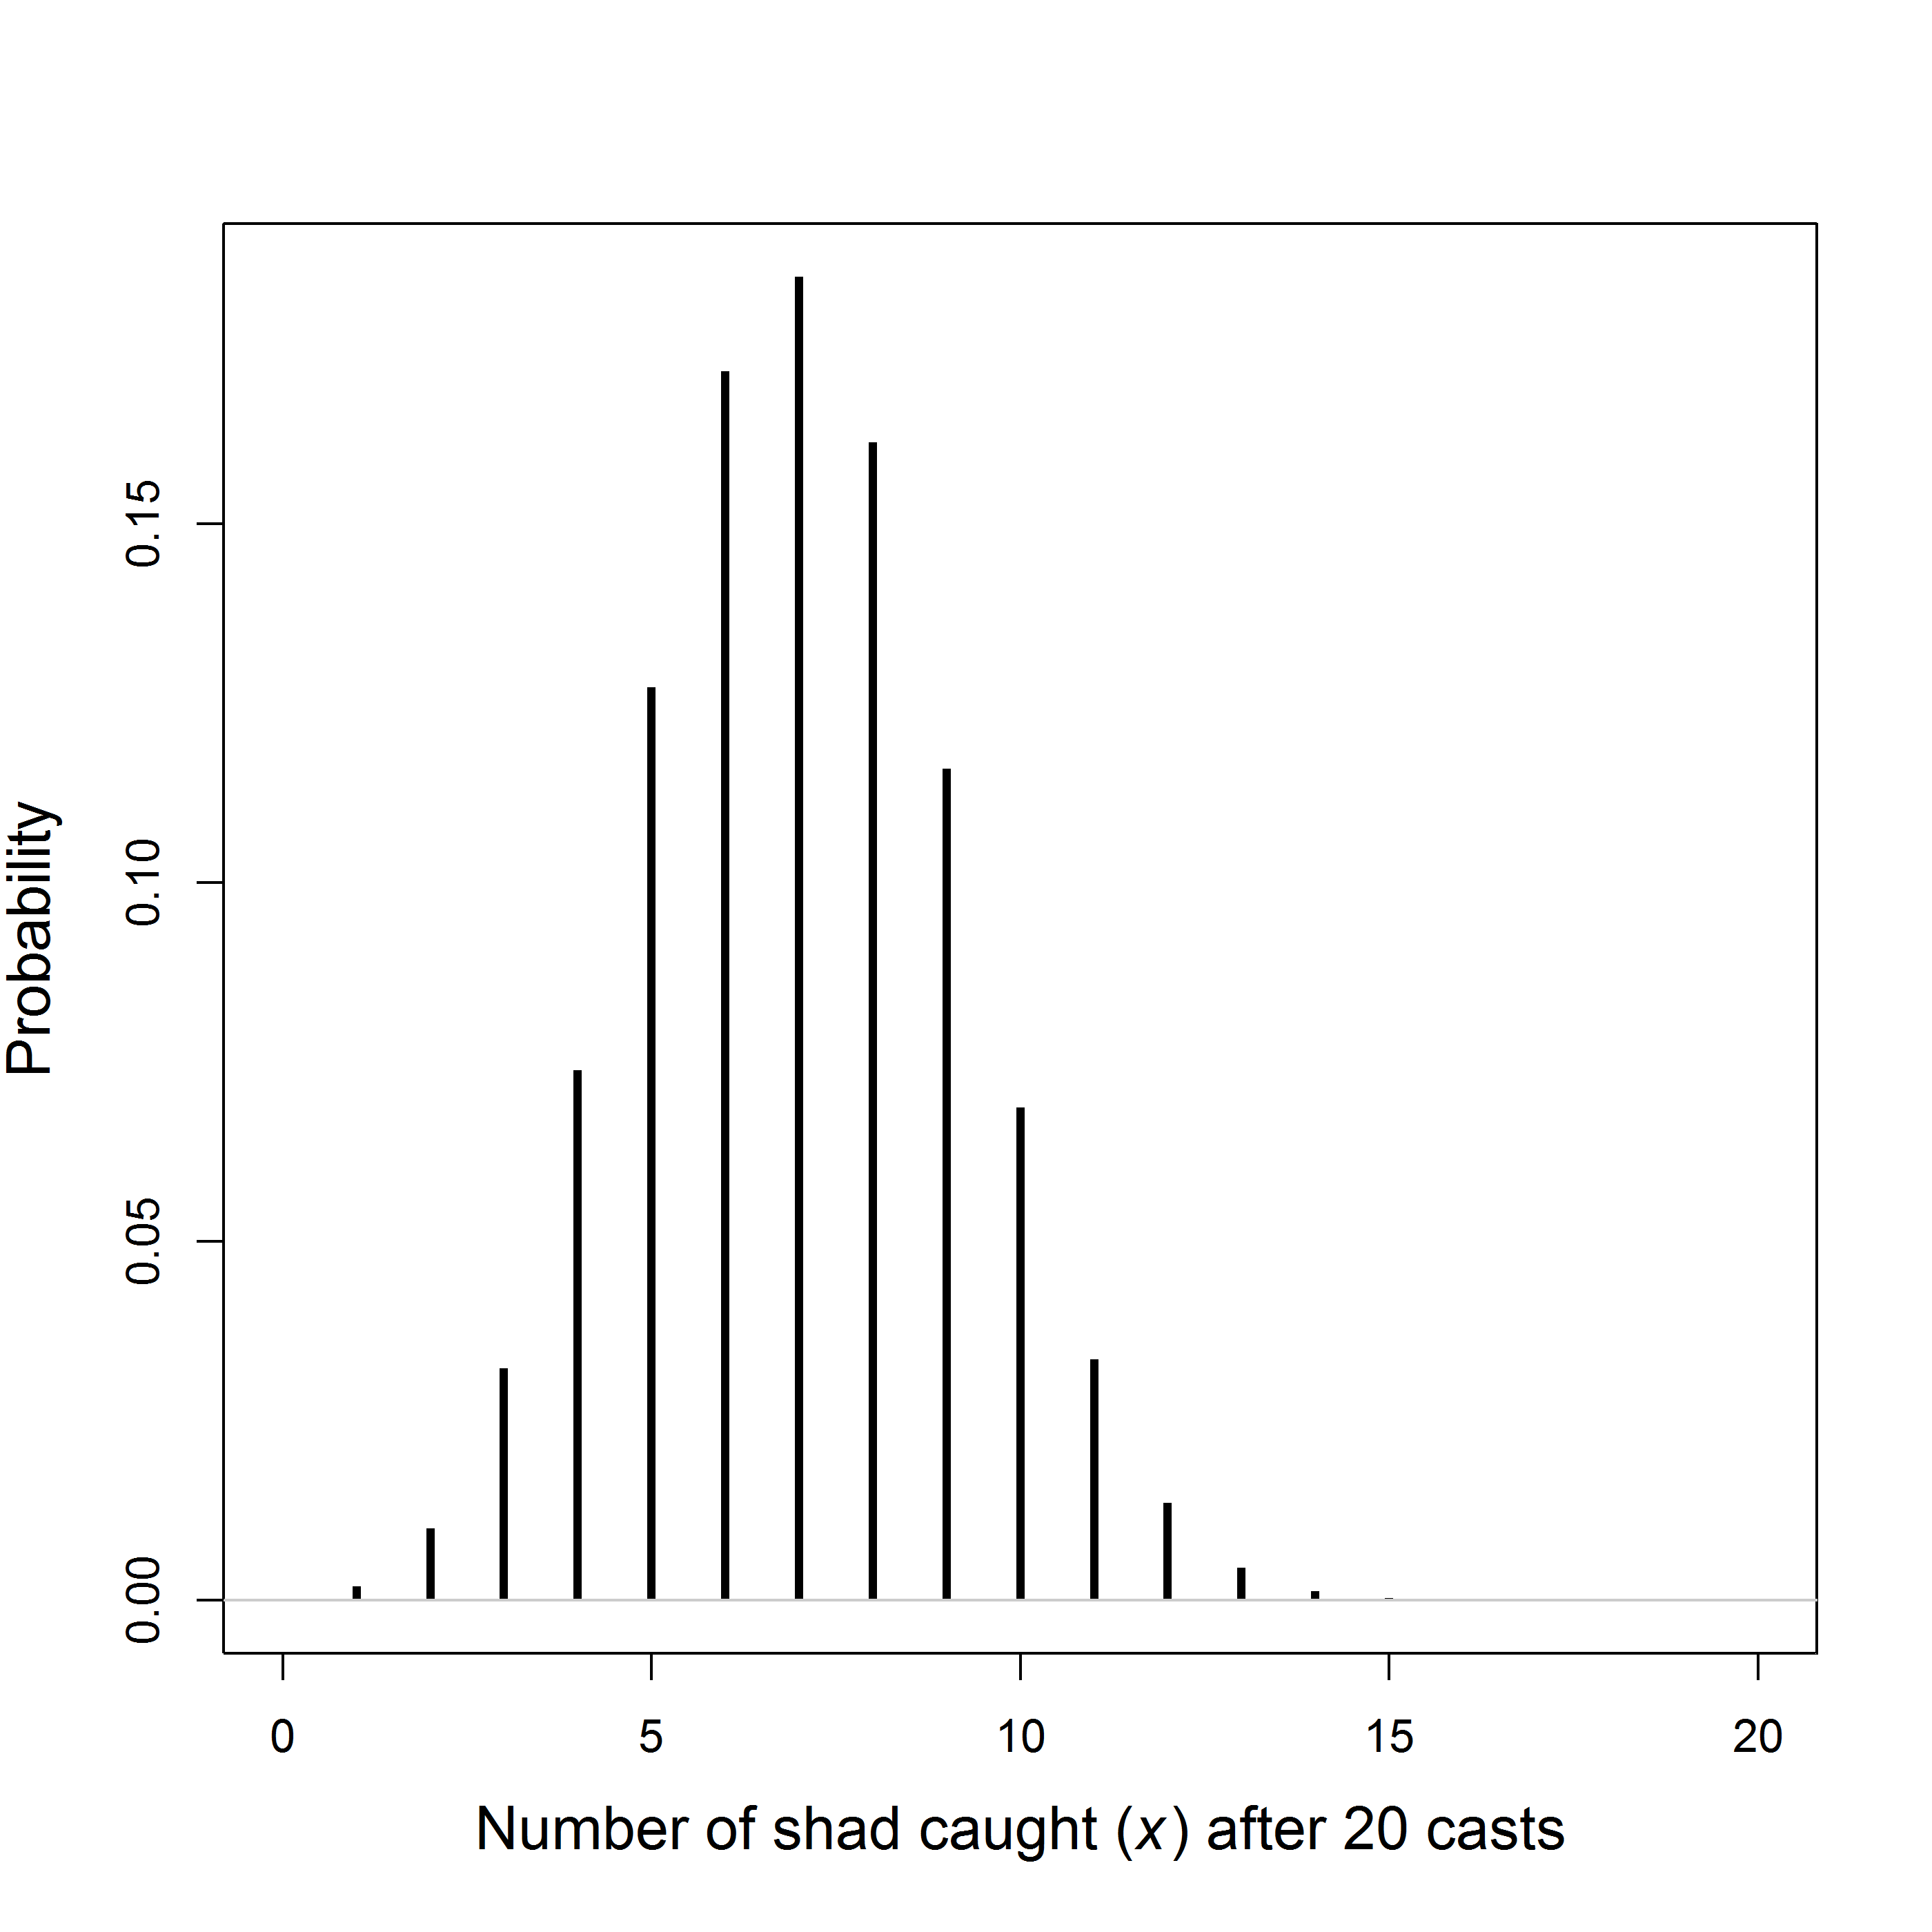
\includegraphics[width=0.65\textwidth]{Ch2/figs/bin}
\caption{The binomial probability mass function with $N=20$ and
  $p=0.35$. }
\label{modeling.fig.bin}
\end{figure}

The purpose of this little example is to show that once we specify a
model for the random variable(s) being studied, we can begin drawing
conclusions, i.e. making inferences, about the processes of interest,
even in the face of uncertainty. Probability distributions are
essential to this process, and thus we need to
understand them in more depth.


%%%% XXXX Add support??
% XXXX Make sideways table?
\begin{table}%[t!]
%  \small
  \caption{Common probability density functions (pdfs) and probability
    mass functions (pmfs) used throughout this book.}
  \begin{tabular}[t]{lcccc}
    \hline
    Distribution & Notation & pmf or pmf & Mean & Variance \\
    \hline
    \multicolumn{5}{c}{Discrete random variables} \\
    Poisson & $x \sim \text{Pois}(\lambda)$ &
    $\exp(-\lambda )\lambda^x/x!$ & $\lambda$ & $\lambda$ \\
    Bernoulli & $x \sim \text{Bern}(p)$ & $p^x(1-p)^{1-x}$ & $p$ &
    $p(1-p)$  \\
    Binomial & $x \sim \text{Bin}(N, p)$ & $\binom{x}{N}p^x(1-p)^{N-x}$
    & $Np$ & $Np(1-p)$  \\
    Multinomial & $\mathbf{x} \sim \text{Multinom}(N, \bm{\pi})$ &
    $\binom{N}{x_1 \cdots x_k}\pi_1^{x_1} \cdots \pi_k^{x_k}$ & $N\pi_k$
    & $N\pi_k(1-\pi_k)$ \\
    \multicolumn{5}{c}{Continuous random variables} \\
    Normal & $x \sim \text{N}(\mu, \sigma^2)$ & $\frac{1}{\sigma\sqrt{2\pi}}
      \exp(-\frac{(x-\mu)^2}{2\sigma^2})$ & $\mu$ & $\sigma^2$  \\
    Uniform & $x \sim \text{Unif}(a, b)$ & $1/(b-a)$ & $(a+b)/2$ &
    $(b-a)^2/12$  \\
%    2D-Uniform & $\mathbf{x} \sim \text{Unif}(\mathcal{S})$ & $1/A(\mathcal{S})$ & &  \\
    Beta & $x \sim \text{Beta}(a, b)$ &
    $\frac{\Gamma(a+b)}{\Gamma(a)+\Gamma(b)}x^{a-1}
    (1-x)^{b-1}$ & $a/(a+b)$ & $\frac{ab}{(a+b)^2(a+b+1)}$ \\
    Gamma & $x \sim \text{Gamma}(a,b)$ &
    $\frac{b^a}{\Gamma(a)}x^{a-1}\exp(-bx)$ & $a/b$ & $a/b^2$  \\
    Multivariate Normal & $\mathbf{x} \sim MVN(\bm{\mu}, \bm{\Sigma})$
    & & & \\
    \hline
  \end{tabular}
  \label{modeling.tab.pdfs}
\end{table}




\subsection{Properties of Probability Distributions}

A pdf or a pmf is a function like any other function
%Probability distributions are functions like any other functions
in the sense that it has one or more arguments whose values determine
the result of the function. However, probability functions have a few
properties that distinguish them from other functions.
The first is that the function
must be non-negative for all possible values of the random variable,
i.e. $[x] \geq 0$. The second requirement is that the integral of
a pdf must be unity, $\int_{-\infty}^{\infty} [x]\, \text{d}{x} = 1$, and similarly
for a pmf, the summation over all possible values is unity, $\sum_x [x]
= 1$. The following \R~code demonstrates
this for the normal and binomial distributions:
%\begin{samepage}
\begin{verbatim}
> integrate(dnorm, -Inf, Inf, mean=0, sd=1)$value
[1] 1
> sum(dbinom(0:5, size=5, p=0.1))
[1] 1
\end{verbatim}
%\end{samepage}
This requirement is important to remember when one  develops a
non-standard probability distribution. For example, in Chapt.
\ref{chapt.state-space} and \ref{chapt.rsf},
we work with resource selection functions whose probability
density function is not one that is pre-defined in software packages
such as \R~or \bugs.

Another feature of probability distributions is that they can be used
to compute important summaries of random variables. The two most
important summaries are the expected value, $\mathbb{E}(x)$,
and the variance $\text{Var}(x)$. The expected value
can be thought of as the average
of a very large sample from the specified distribution. For
example,
one way of approximating the expected values of a binomial
distribution with $K=20$ trials and $p=0.35$ can be implemented in \R~using:
\begin{verbatim}
> mean(rbinom(10000, 20, 0.3))
[1] 6.9865
\end{verbatim}
For most probability distributions used in this book, the expected
values are known exactly, as shown in Table~\ref{modeling.tab.pdfs}, and
thus we don't need to resort to such Monte Carlo approximations. For instance, the
expected value of the binomial distribution is exactly $\mathbb{E}(X) = Kp =
20 \times 0.35 = 7$. In this case, it happens to take an integer
value, but this is not a necessary condition, even for discrete random
variables.

A more formal definition of an expected value is the average of all
possible values of the random variable, weighted by their
probabilities. For continuous random variables, this weighted average
is found by integration: %{\bf XXXX here I put a * for
%  multiplication. Maybe could have a hard space in there to seperate
%  the two pieces XXXXX}
\begin{equation}
  \mathbb{E}(x) = \int_{-\infty}^{\infty} x \times [x] \, \text{d}{x}.
  \label{modeling:eq:EXc}
\end{equation}
For example, if $[x]$ is normally distributed with mean 3 and unit
variance, we could find the expected value using the following code.
\begin{verbatim}
> integrate(function(x) x*dnorm(x, 3, 1), -Inf, Inf)
3 with absolute error < 0.00033
\end{verbatim}
Of course, the mean \textit{is} the expected value of the normal
distribution, so we didn't need to compute the integral but, the
point is, that Eq.~\ref{modeling:eq:EXc} is generic. For discrete
random variables, the expected value is found by summation rather than
integration: %{\bf XXXX same here XXXXX}
\begin{equation}
  \mathbb{E}(x) = \sum_{x} x \times [x]
  \label{modeling:eq:EXd}
\end{equation}
where the summation is over all possible values of $x$.
Earlier we
approximated the expected value of the binomial distribution
with $K=20$ trials and $p=0.35$ by taking a Monte Carlo
average. Eq.~\ref{modeling:eq:EXd} let's
find the exact answer,  using this bit of \R~code:
\begin{verbatim}
> sum(dbinom(0:100, 20, 0.35)*0:100)
[1] 7
\end{verbatim}
This is great. But of what use is it? One very
important concept to understand is that when we fit
%(generalized linear)
models, we are often modeling changes in the expected value of some random
variable. For example, in Poisson regression, we model its expected
value, say $\lambda$,
which may be a function
of environmental variables.

The ability to model the expected value of a random variable gets us
very far, but we also need sometimes a model for the variance of the random
variable. The variance %is itself a type of expected value; one that
describes the amount of variation around the expected
value. Specifically, $\text{Var}(x) = \mathbb{E}((x -
\mathbb{E}(x))^2)$. Clearly, if the variance is zero, the variable is
not random as there is no uncertainty in its outcome.
For some distributions, notably the normal distribution, the variance
is a parameter to be estimated. Thus, in ordinary linear regression,
we estimate both the expected value $\mu=\mathbb{E}(x)$,
which may be a function of covariates, and the variance
$\sigma^2$, or similarly the residual standard error $\sigma$. For
other distributions, the variance is not an explicit parameter to be
estimated, and instead, the mean to variance ratio is fixed. In the
case of the Poisson distribution, the mean is equal to the
variance, $\mathbb{E}(x) = \text{Var}(x) = \lambda$.
%This is often viewed as a restriction because in ecology
%count data often have a variance greater than the mean. However, much
%of this variation can be ``explained'' by modeling the mean as a
%function of covarites. Still, in cases where extra-Poisson variation
%exists, other distributions such as the negative binomial or
%zero-inflated Poisson distribution may be required.
A similar
situation is true for the binomial distribution---the variance is
determined by the two parameters $K$ and $p$, $\text{Var}(x) = Kp(1-p)$. Thus
in our earlier example with $K=20$ and $p=0.35$, the variance is
4.55. Toying around with these ideas using random number generators
may be helpful. Here is some code to illustrate some of these basic concepts:
\begin{verbatim}
> 20*0.35*(1-0.35)             # Exact variance, Var(x)
[1] 4.55
> x <- rbinom(100000, 20, 0.35)
> mean((x-mean(x))^2)          # Monte Carlo approximation
[1] 4.545525
\end{verbatim}



\section{Common Probability Distributions}
\label{sec.modeling.distributions}

We got a little ahead of ourselves in the previous sections by using
the binomial and Poisson distributions without describing them in detail.
A solid understanding of the binomial, Poisson, multinomial, uniform,
and normal (or Gaussian)
distributions is absolutely essential throughout the
remainder of the book. We will occasionally make use of other
distributions such as the %normal (or Gaussian),
beta, log-normal, %multivariate-normal,
gamma, Dirichlet, etc$\dots$ that can be helpful when
modeling capture-recapture data, but these distributions can be
readily understood once you are comfortable with the more commonly
used distributions described in this section.

\subsection{The Binomial Distribution}

The binomial distribution plays a critical role in ecology. It is
used for purposes as diverse as modeling count data, survival
probability, occurrence probability, and capture probability, just to
name a few.
To describe the properties of the binomial distribution, and related
distributions, we will introduce a new example.
Suppose we are conducting a bird survey at a site in which $N=10$
chestnut-sided warblers (\textit{Stetophaga pensylvanica}) occur, and
each of these individuals has a detection probability of $p=0.5$. The
binomial distribution is the natural choice for describing the number
of individuals that we would expect to detect ($n$) in this
situation, and using our notation, we can write the model as: $n \sim
\text{Binomial}(10, 0.5)$. Note that if $p \equiv 1$ and we visit the
site on $K$ occasions, the observations $\{n_1, \ldots, n_K\}$
would not be random outcomes---we would always observe
$n_k=10$. That is, the observed data would exactly equal the expected
value and the variance would be zero.
However, when $p<1$, we can expect that we will observe
a different number of warblers on each replicate visit. To see this,
we can simulate data under this simple model with $K=3$ survey occasions
\begin{verbatim}
> n <- rbinom(3, size=10, prob=0.5) # Generate 3 binomial outcomes
> n                                 # Display the 3 values
[1] 6 4 8
\end{verbatim}
The vector of counts will typically differ each time you issue this
command; however, we know the probability of observing any value of
$n_k$ because it is defined by the binomial pmf. As we demonstrated
earlier, in \R~this probability can be found using the \verb+dbinom+
function. For example, the probability of observing $n_k=5$ is given by:
\begin{comment}
  Without knowing a thing about probability distributions, most people
  would recognize that the expected value of $x_j$ is $10 \times 0.5 =
  5$. That is, the most likely number of chestnut-sided warblers that
  we would expect to detect is 5. In this case, however, we did not
  observe a single 5, but rather observed counts of 6, 4, and 8
  chestnut-sided warblers on the first, second, and third surveys
  respectively. If 5 is the most likely outcome, how likely was it to
  observe these data? And what is the actual probability of observing
  a 5? These questions can all be answered by the probability mass
  function (pmf) for the binomial distribution.

  The probability of
  observing a 5 (or any other number) when $N=10$ and $p=0.5$ can be
  computed in \R~by issue the following command:
\end{comment}
\begin{verbatim}
dbinom(5, 10, 0.5)
\end{verbatim}
This simply evaluates the function shown in
Table~\ref{modeling.tab.pdfs}. We could do the same more transparently, but
less efficiently, using any of the following:
\begin{verbatim}
n <- 5; N <- 10; p <- 0.5
factorial(N)/(factorial(n)*factorial(N-n))*p^n*(1-p)^(N-n)
exp(lgamma(N+1) - (lgamma(n+1) + lgamma(N-n+1)))*p^n*(1-p)^(N-n)
choose(N, n)*p^n*(1-p)^(N-n)
\end{verbatim}
Note that the last three lines of code differ only in how they compute the
binomial coefficient $\binom{N}{n}$, which is the number of different ways
we could observe $n=5$ of the $N=10$ chestnut-sided warblers at the site. The
binomial coefficient, which is read ``N choose n'' is defined as
\begin{equation}
  \label{eq:1}
  \binom{N}{n} = \frac{N!}{n!(N-n)!}.
\end{equation}

Now that we know how to simulate binomial data and compute the
probabilities of observing any particular outcome $n$, conditional on the
parameters $N$ and $p$, we can contemplate the relevance of the
binomial distribution in spatial capture-recapture models. One
important application of the binomial distribution is as a model encounter
frequencies. Indeed, one of the most important encounter models in SCR
will be referred to as the ``binomial encounter model'', in which
% For example, suppose that we operate an array of hair snares for
% $K=4$ survey occasions. In this case, an individual can be
% encountered at most once at a snare during a single occasion (because
% multiple distinct hair deposits cannot be distinguished), but the
% individual can be encountered at multiple snares during an occasion as
% it moves about its home range. If there are no time-varying, or
% occasion-specific, covariates then a natural model for
the number of times individual $i$ is captured at ``trap'' $j$ after
$K$ survey occasions is
modeled as $y_{ij} \sim \text{Binomial}(K, p_{ij})$. Here, $p_{ij}$ is the
encounter probability determined, in part, by the distance between an
animal's activity center and the trap location, as will be described
more fully in subsequent chapters. The important point to note is
that $y_{ij}=0$ if individual $i$ is never encountered at trap $j$,
and $y_{ij}=4$ if it is encountered on all four occasions. This
binomial encounter model is
described in detail in Sec.~\ref{scr0.sec.binomial}.
Another important application of the binomial distribution is as a
prior for the population size parameter in Bayesian analyses, as is
discussed in Chapt.~\ref{chapt.closed}.
% , is somewhat advanced, but
% here we simply note that one must choose a prior distribution for $N$.
% In likelihood analysis a Poisson prior is often used, but when
% conducting a Bayesian analysis, we typically use a practice known as
% data augmentation that results in the prior distribution: $N \sim
% \text{Binomial}(M, \psi)$ where $M$ is an arbitrarily large integer,
% and




\subsection{The Bernoulli Distribution}

%{\bf XXXX Should this come before the binomial? XXXXX}
% ANDY, I guess it could go either way, but I prefer going from
% general to specific in this case. Same goes for multinomial -> categorical

Above, we showed three alternatives to \verb+dbinom+ for evaluating the
binomial pmf. These three commands differed only in how they computed
the binomial coefficient, which we needed because of the numerous ways
in which we could observe $n=5$ given $N=10$. To conceptualize
this, let $y_i$ be a binary variable indicating if individual $i$
was detected or not. Hence, given that 5 individuals were detected,
the vector of individual detections could be something like
$\mathbf{y}=(0,0,1,1,1,1,1,0,0,0)$, which would indicate
that we detected individuals 3-7 but not 1-2 or 8-10. For $N=10$ and
$n=5$, the binomial coefficient tells us that there
are 252 possibilities of vectors $\mathbf{y}$ that have 5 ones. However, when $N \equiv 1$, this term
drops from the pmf and the result is the pmf for the Bernoulli
distribution. That is, the Bernoulli distribution is simply the
binomial distribution when $N \equiv 1$. Alternatively, we could say that the binomial
distribution is the outcome of $N$ $iid$ Bernoulli trials. We use the
standard term ``$iid$'' to mean {\it independent, identicially distributed}.
%% DEFINE iid here?

The utility of the Bernoulli distribution is evident when we imagine
that not all of the chestnut-sided warblers have the same detection
probability. Thus, if some individuals can be detected with
probability 0.3 and others have a 0.7 detection probability, then the
model $n \sim \text{Binomial}(N, p)$ is no longer an accurate
description of system since $p$ is no
longer constant for all individuals. %%%%a scalar, i.e. a single value.

%% FIXME: Need to clean up notation of $J$ visits

To properly account for variation in $p$, we could redefine our model
for the %our notation
%describing how the
counts of chestnut-sided warblers as
%are generated. Our model now is
\begin{gather}
y_{ik} \sim \text{Bernoulli}(p_i) \nonumber \\% \;\; \text{for} \; i=1,2,\dots,N \\
n_k = \sum_{i=1}^N y_{ik}
\label{modeling.eq.Bern}
\end{gather}
This  states that individual $i$ is detected with probability
$p_i$, and the observed count is the sum of the $N$ Bernoulli
outcomes.

An important point is that the individual-specific data $y_{ik}$ can only be
observed  {\it if} the individuals are uniquely distinguishable, such as when they
are marked by biologists with color bands, or by boy-biologists with
paint-ball guns.
%Indeed, this is one of the important
%motivations for capture-recapture studies.
In such cases, the Bernoulli distribution allows us to
model variation in detection probability among individuals and thus
would be preferable to the binomial distribution, which assumes that each
of the $N$ individuals have the same $p$.
For this reason, the Bernoulli
distribution, as simple as it is, is of paramount importance in
capture-recapture models, including spatial capture-recapture models
in which there is virtually always substantial and important variation in capture probability
among individuals. Indeed, it could be said the Bernoulli model is the
canonical model in capture-recapture studies, and most of the
different flavors of capture-recapture models differ primarily in how $p_i$ is
specified. % and how $N$ is estimated.

The Bernoulli pmf is given by  $p^n(1-p)^{1-n}$ and hence we do not need canned
functions to facilitate its evaluation. Of course, if you wanted to, you
could always use \verb+dbinom+ with the \verb+size+ argument set to
1, e.g. \verb+dbinom(1, 1, 0.3)+ returns the Bernoulli probability of
observing $n=1$ given $p=0.3$.

\subsection{The Multinomial and Categorical Distributions}
\label{modeling.sec.multinom}

The binomial distribution is used
when we are accumulating a binary response -- that is, one in which there are two possible categories, such as success/failure or captured/not-captured.
The multinomial distribution is a multivariate extension of
the binomial used when there are $G>2$ categories.
The multinomial distribution can be thought of as a model for placing
$N$ items in the $G$ categories, which are also called bins or cells. Each bin has
its own probability $\pi_g$ and these probabilities must sum to one.
In ecology, $N$ is often population size or the number of individuals
detected, but the definition of the $G$ bins varies among
applications. For example, in distance sampling, when the distance
data are aggregated into intervals,
the bins are the distance intervals, and the cell probabilities are
functions of detection probability in each interval \citep{royle_etal:2004}.

The multinomial distribution is widely used to model data from traditional,
non-spatial capture-recapture studies.
Earlier we let $y_{ik}$ denote a binary random variable indicating if
warbler $i$ was detected on survey $k$. The vector of observations for an
individual, $\mathbf{y}_i$, is often referred to as the individual's
``encounter history''. The number of possible encounter
histories depends on the number of survey occasions. Specifically,
there are $2^K$
possible encounter histories\footnote{When $N$ is unknown, we can
  never observe the ``all-0'' encounter history, corresponding
to an individual that is not
  detected, and thus the number of ``observable'' encounter histories
  is $2^{K-1}$}.
If we tabulate the number of individuals with each encounter history,
the frequencies can be modeled using the multinomial
distribution. %, as we will soon explain.

Going back to our
chestnut-sided warbler example, suppose the 10 individuals are marked
and we make $K=2$ visits to the site such that there are $2^K = 4$ possible encounter
histories: $(11, 10, 01, 00)$, where, for example,  ``10'' is the
encounter history for an individual detected on the first visit but not
the second. If $p=1$, then the
encounter history for each of the 10 individuals must  be ``11''. That
is, we would detect each individual on both occasions. In this case,
we could format our data as $\mathbf{h} = (10, 0, 0, 0)$. The
corresponding cell probabilities would be $\bm{\pi} = (1, 0, 0,
0)$. What about the situation where $p<1$, e.g. $p=0.3$? In this case, the
probability of observing the capture history ``11'' (detected on both
occasions) is $p \times p = 0.3 \times 0.3 = 0.09$. The probability of
observing ``10'' is $p \times (1-p) = 0.21$. Following this logic, the vector
of cell probabilities is $\bm{\pi} = (0.09, 0.21, 0.21, 0.49)$. We can
simulate data under this model as follows: 
\begin{verbatim}
> caphist.probs <- c("11"=0.09, "10"=0.21, "01"=0.21, "00"=0.49)
> drop(rmultinom(1, 10, caphist.probs))
11 10 01 00
 0  3  2  5
\end{verbatim}
(the \verb+drop+ function simply converts the matrix to a vector).
The
result of our simulation is that zero individuals were observed with
the capture history ``11'' and 5 individuals were observed with the
capture history ``00''. The other 5 individuals were observed one out
of the two occasions. This is not such a surprising outcome given
$p=0.3$.
%Note that the a single outcome of a multinomial distribution
%is a vector, and hence it is a multivariate distribution in contrast
%to the univariate distributions discussed so far.

As in non-spatial capture-recapture studies, the multinomial
distribution turns out to be very important in spatial
capture-recapture studies. However, $N$ is not defined as population
size. Rather, we use the multinomial distribution when an individual
can only be captured in a single trap during an occasion. Thus
$N=1$ and the cell probabilities are the probabilities of
being captured in each trap. A thorough discussion of this point can
be found in Chapt.~\ref{chapt.poisson-mn}. Another application of the
multinomial distribution in SCR models is discussed in
Chapt.~\ref{chapt.state-space} where we discuss how to model the
probability that an individual's activity center is located in one of
the cells of a raster defining the spatial region of interest.

%It is worth noting that,
Just as the Bernoulli distribution is the elemental form of the
 binomial distribution (being the case $N=1$), the
categorical distribution is essentially equivalent to
%special case of
the multinomial distribution with size parameter
$N\equiv1$. The only difference is that, rather than returning a
vector with a single element equal to 1, it returns the element number
where the 1 occurs. For example, if $\mathbf{y}=(0,0,1,0)$ is an outcome of a
multinomial distribution with $N=1$, then the categorical outcome
would be 3 because the 1 is located in third position in the vector. Thus, in spatial
capture-recapture models, we might use either the multinomial
distribution with $N=1$ or %we can just as well use
the categorical distribution. %They are equivalent.
The various {\bf BUGS} engines describe the categorical distribution
by the declaration \mbox{\tt dcat} and, in {\bf R}, we can simulate
categorical outcomes using the function \mbox{\tt sample}.


\subsection{The Poisson Distribution}


The Poisson distribution is the canonical model for count data in
ecology.  More generally, the
Poisson distribution is a model for random variables taking on
non-negative, integer values.  Although it is a simple model having just one
parameter, $\lambda = \mathbb{E}(x) = \text{Var}(x)$, its applications
are highly diverse, including
as a model of spatial variation in abundance or as a model for the
frequency of behaviors over time.  Just as logistic regression is the
standard generalized linear model (GLM) used to model binary data, Poisson
regression is the default GLM for modeling count data and variation in
$\lambda$.

The Poisson distribution is related to
both the binomial and multinomial distributions, and the following two
bits of trivia are occasionally worth knowing. First, it is the limit of the binomial
distribution as $N \to \infty$ and $p \to 0$, which means that for
high values of $N$ and low values
of $p$, $\text{Poisson}(N\times p)$ is approximately equal to $\text{Binomial}(N,
p)$. Second, if $\{n_1 \sim \text{Poisson}(\lambda_1),
%n_k \sim \text{Poisson}(\lambda_k),
\dots, n_K \sim \text{Poisson}(\lambda_K)\}$
then the vector of counts is multinomial, $\{n_1, \dots, n_K\}
\sim \text{Multinomial}(\sum_k n_k, \{\frac{\lambda_1}{\sum_k \lambda_k},
%\frac{\lambda_k}{\sum_{n_k} \lambda_k},
\dots, \frac{\lambda_K}{\sum_k \lambda_k}
\})$.

The Poisson distribution has two important uses in spatial
capture-recapture models: (1) as a prior distribution for the
population size parameter $N$, and (2) as a model for the frequency of
captures in a trap. In the first context, the Poisson prior for $N$
results in a Poisson point process for the location of the $N$
activity centers in the region of interest. This topic is discussed
in-depth in Chapt.~\ref{chapt.scr0} and Chapt~\ref{chapt.state-space}.
% point process model, which is a
% spatially-explicit extension of the simple Poisson model.
% If $N$ individuals are uniformly distributed in some region
% $\mathcal{S}$ with area $A$, and $N$ is a Poisson
% random variable, we call this the homogeneous Poisson point process
% whose intensity parameter is $\lambda = 1/A$. The intensity parameter
% is defined as the expected number of points that one would find in an
% infinitesimally small area. Often, the intensity parameter is not
% constant, but rather it takes on different values for each location
% $x$ in the region $\mathcal{S}$. The inhomogeneous Poisson point
% process model can be useful in such cases, and typically, the
% intensity is modeled as a log-linear function of spatially-referenced
% environmental covariates. Thus, rather than $\lambda$, the intensity
% parameter is now $\lambda(x)$. Inhomogeneous Poisson point process
% models have a long history of applications in forestry, and are now
% being increasingly used to model species distributions. They are also
% extremely important in spatial capture-recapture as we will soon see.
% Under the homogeneous Poisson point process model,
% the number of individuals occurring in some
% region $B \in A$ is Poisson distributed with expectation
% $\lambda = N/A$. As before, $\lambda$ might vary among regions, which
% might be distinct habitat patches or arbitrarily-defined survey plots or
% quadrats and Poisson regression could be used for inference.
The second use of the Poisson distribution in spatial capture-recapture is
to describe data from sampling methods in which an
individual can be detected multiple times at a trap during a single
occasion. For example, in camera trapping studies we might obtain
multiple pictures of the same individual at a trap during a single sampling
occasion. Thus, $\lambda$ in this case would be defined as the
expected number of detections or captures per occasion.


\subsection{The Uniform Distribution}

The %first continuous distribution we will describe is the
lowly uniform distribution is a continuous distribution whose
only two parameters are the lower and upper bounds that restrict the
possible values of the random variable $x$. These bounds
are almost always known, so there is typically nothing to
estimate. Nonetheless, the uniform
distribution is one of the most widely used distributions,
especially among Bayesians who frequently use it to as a ``non-informative''
prior distribution for a parameter. For example, if we
have a capture probability parameter $p$ that we wish to estimate, but
we have no prior knowledge of what value it may take in the range
[0,1], we will often use the prior $p \sim \text{Uniform}(0,1)$. This
states that $p$ is equally likely to take on any value between
zero and one.

Another common usage of the uniform distribution is as a prior for the
%x- and y-
coordinates of points in the real plane, i.e. in two-dimensional
space. Such a use of the uniform distribution implies that a point process is
``homogeneous'', meaning that the location of one point does not
affect the location of another point and that the expected density of
points is constant throughout the region. Thus, to simulate a
realization from a homogeneous Poisson point process in the unit square
$[0,1] \times [0,1]$, we could use the following \R~code:
\begin{verbatim}
D <- 100    # points per unit area
A <- 1      # Area of unit square
N <- rpois(1, D*A)
plot(s <- cbind(runif(N), runif(N)))
\end{verbatim}
where \verb+s+ is a matrix of coordinates with $N$ rows and 2 columns. We
will often represent the uniform point process using the following notation:
\begin{equation}
  {\bf s} \sim \text{Uniform}(\mathcal{S})
\end{equation}
where ${\cal S}$ is some specific unit of space called the state-space
of the random variable ${\bf s}$.
It would be more correct to somehow distinguish this
two-dimensional uniform distribution for the univariate one. That is,
it might be more clear to use notation such as
${\bf s} \sim \text{Uniform}_2(\mathcal{S})$ instead, but this is somewhat
cumbersome, so we will opt for the former expression.


%\subsection{The Normal and Bivariate Normal Distributions}
\subsection{Other Distributions}

The other continuous distributions that are regularly encountered in SCR
models are
primarily used as priors in Bayesian analyses, and thus we will avoid
a lengthy discussion of their properties. %The  we will briefly
%cover here are the beta and gamma distributions, which are
%particularly useful as priors for probabilities and positive-valued
%parameters respectively. Although we will keep it very brief, note that
%Table~\ref{modeling.tab.pdfs} includes
%the pdfs, expected values, and variances of these distributions.
%A more thorough treatment of
%these distributions can be found in \citet{link_barker:2010}.
%This might seem odd given that
%standard statistics courses taken by ecologists focus heavily on the normal
%distribution. However, in capture-recapture studies, we rarely observe
%random variables that are continuous,
%and hence, we will just briefly
%mention the normal, beta, and gamma distributions.
%Once upon a time, ecologists modeled just about everything as normally
%distributed. One reason for this is that methods such a linear
%regression and $t$-tests were all that were available in many
%primitive stats software programs. Another reason why
The normal distribution, also called the Gaussian
distribution, is perhaps the most widely recognized and applied probability model in
statistics, but it plays only a minor role in SCR models although it
has been used as a model for signal strength in acoustic SCR models
\citep{efford_etal:2009ecol,dawson_efford:2009}, and see Sec. \ref{poisson-mn.sec.acoustic}. %The reason
%being that many of the random variables in SCR models are discrete,
%and distinctly not normally distributed.
Nonetheless, it
is the canonical prior for any continuous random variable with
infinite support, and thus it is often used as a prior when applying Bayesian
methods. One common usage is as a prior for the $\beta$
coefficients of a linear model defining some parameter as a function
of covariates (usually on a transformed scale). An example, including a
cautionary note, is provided in Sec.~\ref{glms.sec.choice}.
Be aware that although the normal distribution is typically
parameterized in terms of the variance parameter $\sigma^2$, in
the \bugs~language, the inverse of the variance, or precision, is used
instead, $\tau = 1/\sigma^2$.

The bivariate normal distribution is a generalization of the
normal distribution and a special case of the multivariate normal
distribution whose pdf is shown in Table~\ref{modeling.tab.pdfs}. The
bivariate normal distribution is used to model two (possibly) dependent
continuous variables whose symmetric variance-covariance matrix is
denoted $\bm{\Sigma}$.
%The parameter $\rho$ is two off-diagonals of this matrix are
In SCR models, we most often use this model as
a rudimentary description of movement outcomes about a home range
center. If there is there is no correlation, then the model reduces to
two independent normal draws along the coordinate axes. The following code generates bivariate normal
outcomes with no correlation ($\rho=0$, the object \verb+X1+) and with
$\rho=0.9$, the object \verb+X2+.
\begin{verbatim}
library(mvtnorm)
set.seed(3)
mu <- c(0,0)
Sigma <- matrix(c(1, .9, .9, 1), 2, 2)
X1 <- cbind(rnorm(50, mu[1], Sigma[1,1]), # No correlation (rho=0)
            rnorm(50, mu[2], Sigma[2,2]))
X2 <- rmvnorm(50, mu, Sigma)              # rho=0.9
\end{verbatim}
Fig.~\ref{modeling.fig.bvn} shows the simulated points.
\begin{figure}
  \centering
  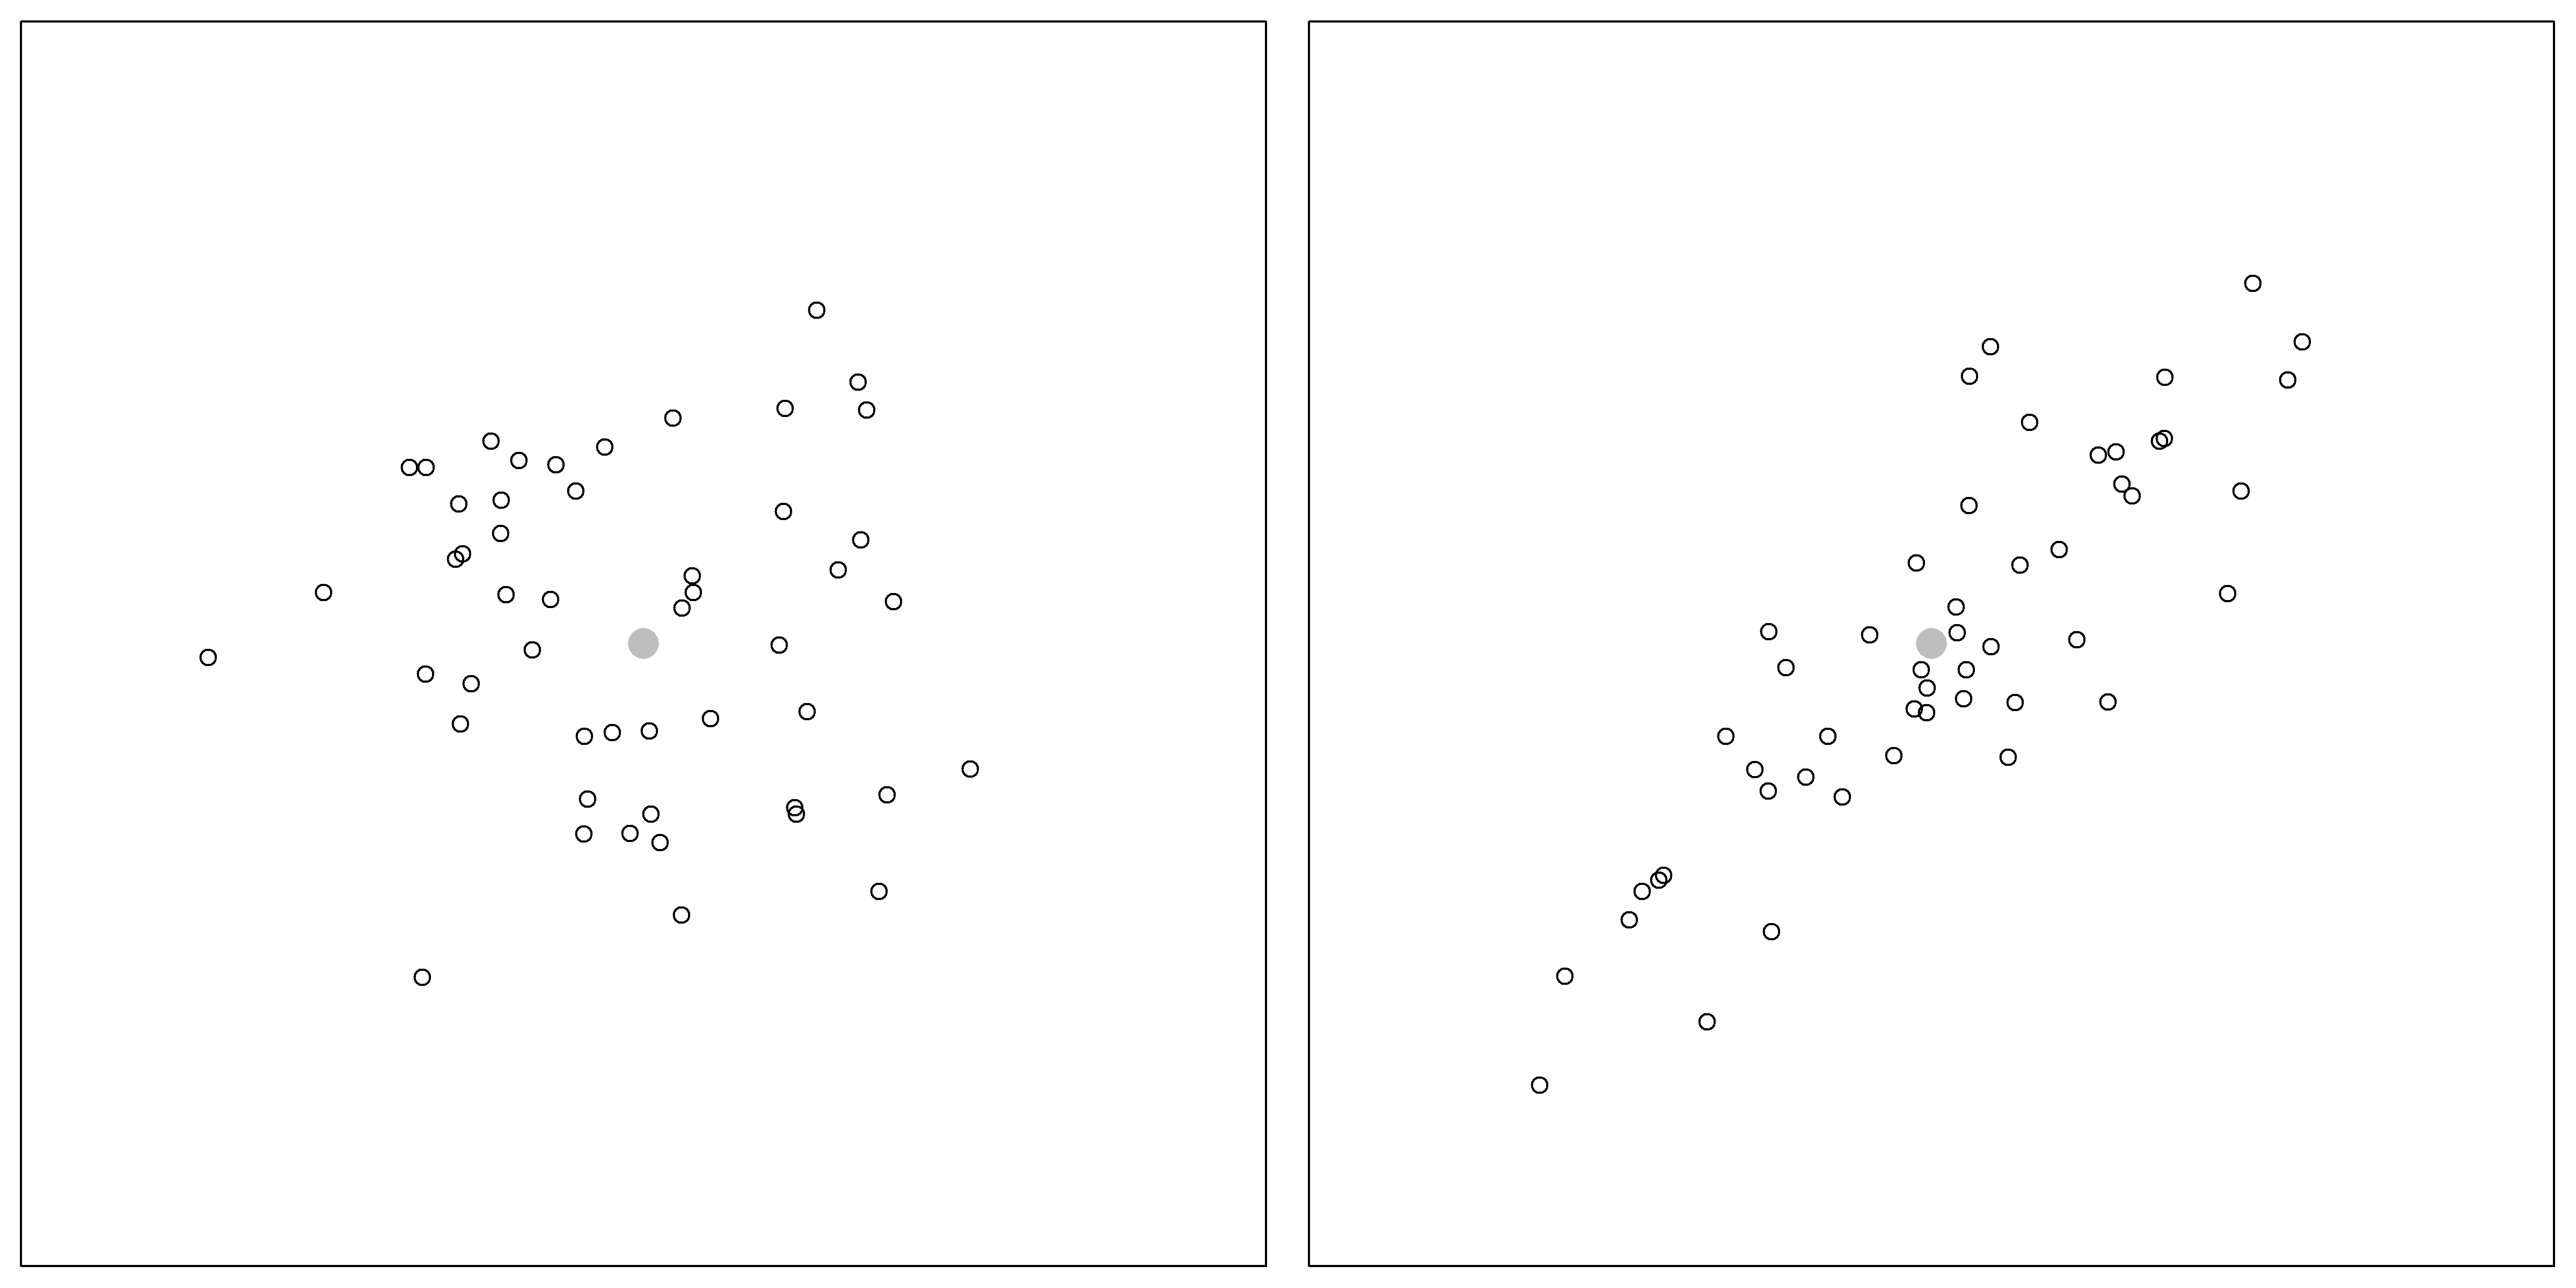
\includegraphics[width=0.9\textwidth]{Ch2/figs/bvn}
  \caption{Two realized point patterns from the bivariate normal distribution. }
  \label{modeling.fig.bvn}
\end{figure}

Several of the parameters in capture-recapture models do not have
infinite support, but are instead are
probabilities restricted to the range $[0,1]$, or are positive valued
living between zero and $\infty$. The beta distribution is the
standard prior used for probabilities because it can be used to express either a
lack of knowledge or very precise knowledge about a
parameter. For example, a $\text{Beta}(1,1)$ distribution is
equivalent to a $\text{Uniform}(0, 1)$ distribution. However, unlike the
the uniform distribution, the beta distribution can be used as an
informative prior; for example if published estimates of detection
probability exist we can choose parameters of the beta distribution to
reflect that. To gain some familiarity with the beta
distribution, execute the following \R~commands:
\begin{verbatim}
curve(dbeta(x, 1, 1), col="black", ylim=c(0,5))
curve(dbeta(x, 10, 10), col="blue", add=TRUE)
curve(dbeta(x, 10, 20), col="darkgreen", add=TRUE)
\end{verbatim}

Other parameters in SCR models are continuous but
positive-valued and can be modeled using the gamma distribution. As
with the beta distribution, the gamma distribution is typically
favored over the uniform distribution when one is interested in using
an informative prior. It is also frequently used as a vague prior for
the inverse of
variance parameters, but it is wise to compare this prior to a uniform
to assess its influence on the posterior.

\section{Statistical Inference and Parameter Estimation}

If the parameters of a statistical model were known with absolute
certainty, then it would be possible to
%could ignore statistial inference a
use pdfs and pmfs to make direct
probability statements about unknowns such as future outcomes. However, we
almost never know the actual values of parameters, and instead we have
to estimate them from observations (i.e., data). Our inferences must then acknowledge the uncertainty
associated with our imperfect knowledge of the parameters. Doing so is
most often accomplished using one of two approaches:
classical (frequentist) inference or Bayesian
inference.
%Both types of statistical inference make heavy use of
%probability distributions.
These two modes of inference
regard the uncertainty about parameters in
entirely different ways. In the next chapter, we will review some of
the important concepts in Bayesian inference, so here, we will
focus on the frequentist perspective.

%In classical inference, if
Suppose  we count oak trees at
$J$ sites, and the resulting data $\{y_1, \ldots, y_J\}$ can be
assumed to be iid outcomes from some %  we want to know the average number of oaks
%per site. We might assume that the counts are distributed according to some
distribution, such as the Poisson with unknown parameter $\lambda$. We
want to estimate this parameter. %,
%which is the parameter we need to estimate.
In classical inference, the only uncertainty about $\lambda$ %that we are concerned with
is that attributable to
sampling. For instance, we can imagine repeatedly sampling the
population (sites in this example) and obtaining sample-specific estimates of
$\lambda$. Typically, we entertain the idea that there are an infinite
number of possible samples and so we could obtain an infinite
number of estimates: \{$\hat{\lambda}_1, \hat{\lambda}_2, \hdots,
\hat{\lambda}_\infty\}$. If
these estimates are produced using the method of maximum likelihood,
the distribution of estimates, called the sampling distribution, will
be normally distributed with $\mathbb{E}(\hat{\lambda})=\lambda$. The
standard deviation of the sampling distribution is called the standard
error, which can  be estimated as part of the maximum likelihood
procedure. Given $\hat{\lambda}$ and an estimate of its standard
deviation, we can construct a confidence interval
that will include the true value of $\lambda$  with some prescribed
coverage probability.
%which will tend toward zero as the sample size $J$ increases toward
%infinity. In other words, if the sample size is large, the estimate
%will always be close to the actual parameter value. Maximum likelihood
%is a method of estimating both $\lambda$ and the standard error (or
%variance) of lambda.
%variance of the sampling distribution
%{\bf XXXX not sure sampling distribution was defined yet XXXXX}
%will approach zero as the size of the sample increases towards
%infinity.
Note that there is
no uncertainty associated with the actual parameter---it is regarded
as a fixed value, and hence probability is only used to characterize
the estimator via its sampling distribution.

Maximum likelihood is heuristically a method of finding the most ``likely''
value of $\lambda$, given the observed data, and of characterizing the
variance of the sampling distribution. Of course, it also applies to
cases where the observations are multivariate, or the probability
distribution is a function of multiple parameters. Endless numbers of
textbooks and online resources are available for those interested in a
detailed explanation of maximum likelihood. For our purposes, we wish
to keep it simple and focus on \textit{how} to do it. The first step
is to define the likelihood function, which is
is the joint distribution of the data regarded as a function of
the parameter(s). If the joint distribution of the observations is
denoted by $[y_1, y_2, \dots, y_n | \lambda]$, we usually denote the
likelihood by flipping the arguments:
$\mathcal{L}(\lambda | \mathbf{y}) = [\lambda | y_1, y_2, \dots, y_n]$.

If the observations are $iid$, the likelihood simplifies to
\begin{equation}
  \mathcal{L}(\lambda | \mathbf{y}) = \prod_i [y_i | \lambda].
  \label{modeling.eq.like}
\end{equation}
where $[y_i | \lambda]$ is a probability distribution, like those
discussed in the previous sections. For example, if $y_i$ is
Poisson distributed, then
$[y_i | \lambda] = \text{Poisson}(\lambda) = \frac{\lambda^{y_i}e^{-\lambda}}{y_i!}$.
Although likelihoods are typically shown on the natural scale, we
almost always maximize the logarithm of the likelihood to
avoid computational problems that arise when multiplying very small
probabilities. Thus, we rewrite~\ref{modeling.eq.like} as
\begin{equation}
  \ell(\lambda | \mathbf{y}) = \sum_i \log(f(y_i | \lambda))
  \label{modeling.eq.like2}
\end{equation}
Here is some simple \R~code to simulate independent Poisson outcomes
and estimate $\lambda$ (as though we did not know it) using the
method of maximum likelihood. Actually, we will minimize the negative
log-likelihood because it is equivalent and is the default for \R's
optimizers like \verb+optim+ and \verb+nlm+.
\begin{verbatim}
> lambda <- 3                 # Actual parameter value
> y1 <- rpois(100, lambda)    # Realized values (data)
> negLogLike1 <- function(par) -sum(dpois(y1, par, log=TRUE))
> starting.value <- c(`lambda'=1)
> optim(starting.value, negLogLike1)$par # MLE
  lambda
3.039844
\end{verbatim}
Explicitly maximizing the likelihood, numerically, isn't actually
necessary here because the MLE of
$\lambda$ is given by the  mean of the observations. A more interesting
example is when there are
covariates of $\lambda$. For example, suppose $\lambda$ is a function
of elevation and vegetation height according to: $\log(\lambda_i) =
\beta_0 + \beta_1\texttt{ELEV}_i + \beta_2\texttt{VEGHT}_i$. This is a
standard Poisson regression problem, with likelihood:
\begin{equation}
  \mathcal{L}(\bm{\beta} | \mathbf{y}) = \prod_i \text{Poisson}(y_i | \lambda_i)
  \label{modeling.eq.like3}
\end{equation}
This likelihood is almost identical to the previous one except
that $\lambda$ is now a function, and so we need to estimate the
parameters of the function, i.e. the $\beta$'s. %This class of models is
%known as Poisson regression, a form of a generalized linear model that
%we alluded to earlier.
Some code to fit this model to simulated data is shown here:
\begin{verbatim}
> nsites <- 100
> elevation <- rnorm(100)
> veght <- rnorm(100)
> beta0 <- 1
> beta1 <- -1
> beta2 <- 0
> lambda <- exp(beta0 + beta1*elevation + beta2*veght)
> y2 <- rpois(nsites, lambda)
> negLogLike2 <- function(pars) {
+     beta0 <- pars[1]
+     beta1 <- pars[2]
+     beta2 <- pars[3]
+     lambda <- exp(beta0 + beta1*elevation + beta2*veght)
+     -sum(dpois(y2, lambda, log=TRUE))
+ }
> starting.values <- c('beta0'=0, 'beta1'=0, 'beta2'=0)
> optim(starting.values, negLogLike2)$par
      beta0       beta1       beta2
 0.98457756 -1.03025173 -0.01218292
\end{verbatim}
We see that the maximum likelihood estimates (MLEs) are very close to
the true parameter values.

\begin{comment}
  There are a couple of other basic points to make with respect to
  this example. First, note that, although the log-link is the most commonly used link
  funciton in Poisson regression, many other functions can be
  considered that map the linear predictor (i.e. the righthand side of
  the equation) to the admissible values of the parameter. For example,
  in logistic regression common link distributions include the logit,
  probit, and complementary log-log links. In spatial
  capture-recapture models we often model model capture probability
  using the logit link, although many other options are routinely
  considered. A second think to note is that categorical variables can
  be easily included in the model as covariates. To do so, we simply
  need to create ``dummy variables'' which are combinations of binary
  indicator variables that code each level of the variable.
\end{comment}

In these examples, the parameters we estimated are called fixed
effects by frequentists. Fixed effects are parameters that are not
%themselves
regarded as being random variables.
%\footnote{Thus, technically speaking, there are no such
%  things as fixed effects in Bayesian inference}.
A random effect, in
contrast, is a parameter that can be regarded as the outcome of
a random variable. For instance,
we could entertain the idea that the intercept of our GLM differs
among locations, and that it's actual value is an outcome of a normal
distribution with parameters $\mu$ and $\sigma^2$. In this case,
$\beta_i$ would be a random effect, and our model could be written:
\begin{gather*}
y_i \sim \text{Poisson}(\lambda_i) \\
\log(\lambda_i) = \beta_i + \beta_1\text{ELEV}_i + \beta_2\text{VEGHT}_i \\
\beta_i \sim \text{Normal}(\mu, \sigma^2)
\end{gather*}
This is an example of a mixed effects model or a hierarchical
model. How do we estimate the parameters of a model that includes
random effects? Earlier the likelihood function was written as the
product of probabilities determined by a single pmf or pdf,
$[y|\lambda]$, but now we have an additional random variable, and we
are forced to think about conditional relationships, because $y$
depends upon $\beta_i$ and $\beta_i$ depends upon other parameters,
specifically $\mu$ and $\sigma^2$.
This type of conditional dependence among parameters is the essence of hierarchical
models, and statistical analysis of hierarchical models requires that
we discuss joint distributions, marginal distributions and conditional
distributions.




\section{Joint, Marginal, and Conditional Distributions}

So far we have restricted our attention to situations in which we wish
to make inference about a single random variable.
However, in ecology, we often are interested in multiple random
variables and how they are related.
Let $Y$ be a random variable
%whose realized values
that may or may not be independent of $X$ (here again we will
distinguish between random variables and realized values for
conceptual clarity). Inference
about these two random variables can be made using the joint,
marginal, or conditional distributions---or, we may make use of all of
them depending on the question being asked. In the case of
discrete random variables, the joint
distribution is the probability that $X$ takes on the value $x$
\textit{and} that $Y$ takes on the value $y$, which is written
$[X=x,Y=y]$. To clarify this concept, let's go back to our original
example where $X$ was the number of fish caught after 20 casts, which
we said was an $iid$
binomial random variable. Now,
let's suppose that $X$ depends on the random variable $Y$, which is
the number of other fisherman at the hole. Specifically, let's say
that the probability of catching a fish $p$ is related to $X$
according to $\text{logit}(p) = -0.6 + -2y$. Furthermore, let's
make the intuitive assumption that the number of fishermen at the hole
is a Poisson random variable with mean $0.6$, i.e. $X \sim
\text{Poisson}(0.6)$. Our model is now fully specified, and so we can
answer the question: ``what is the probability of catching $x$ fish
\textit{and} of there being $y$ fishermen at the hole''. This joint
distribution is given by the product of the binomial pmf (with $p$
determined by $y$) and the Poisson pmf with $\lambda=0.6$. The
following \R~code creates the joint distribution.
\begin{small}
\begin{verbatim}
> X <- 0:20  # All possible values of X
> Y <- 0:10  # All possible values of Y
> lambda <- 0.6
> p <- plogis(-0.62 + -2*Y) # p as function of Y
> round(p,2)
 [1] 0.35 0.07 0.01 0.00 0.00 0.00 0.00 0.00 0.00 0.00 0.00
> joint <- matrix(NA, length(X), length(Y))
> rownames(joint) <- paste("X=", X, sep="")
> colnames(joint) <- paste("Y=", Y, sep="")
>
> # Joint distribution [X,Y]
> for(i in 1:length(Y)) {
+     joint[,i] <- dbinom(X, 20, p[i]) * dpois(Y[i], lambda)
+ }
> round(joint,2)
      Y=0  Y=1  Y=2  Y=3 Y=4 Y=5 Y=6 Y=7 Y=8 Y=9 Y=10
X=0  0.00 0.08 0.08 0.02   0   0   0   0   0   0    0
X=1  0.00 0.12 0.02 0.00   0   0   0   0   0   0    0
X=2  0.01 0.08 0.00 0.00   0   0   0   0   0   0    0
X=3  0.02 0.04 0.00 0.00   0   0   0   0   0   0    0
X=4  0.04 0.01 0.00 0.00   0   0   0   0   0   0    0
X=5  0.07 0.00 0.00 0.00   0   0   0   0   0   0    0
X=6  0.09 0.00 0.00 0.00   0   0   0   0   0   0    0
X=7  0.10 0.00 0.00 0.00   0   0   0   0   0   0    0
X=8  0.09 0.00 0.00 0.00   0   0   0   0   0   0    0
X=9  0.06 0.00 0.00 0.00   0   0   0   0   0   0    0
X=10 0.04 0.00 0.00 0.00   0   0   0   0   0   0    0
X=11 0.02 0.00 0.00 0.00   0   0   0   0   0   0    0
X=12 0.01 0.00 0.00 0.00   0   0   0   0   0   0    0
X=13 0.00 0.00 0.00 0.00   0   0   0   0   0   0    0
X=14 0.00 0.00 0.00 0.00   0   0   0   0   0   0    0
X=15 0.00 0.00 0.00 0.00   0   0   0   0   0   0    0
X=16 0.00 0.00 0.00 0.00   0   0   0   0   0   0    0
X=17 0.00 0.00 0.00 0.00   0   0   0   0   0   0    0
X=18 0.00 0.00 0.00 0.00   0   0   0   0   0   0    0
X=19 0.00 0.00 0.00 0.00   0   0   0   0   0   0    0
X=20 0.00 0.00 0.00 0.00   0   0   0   0   0   0    0
\end{verbatim}
\end{small}
This matrix tells us the probability of all possible combinations of
$x$ and $y$, and we see that the most likely value is $(X=1,Y=1)$,
i.e. we will catch 1 fish and there will be 1 other fisherman. This
matrix also demonstrates the law of total probability, which dictates
that the sum of of these probabilities must equal 1.

Perhaps most fisherman don't care about joint distributions, but a
question that might be asked is ``what is the probability
of catching 1 fish today?'' We know that this depends on the
number of fisherman, but we don't know how many will show up
today, so this is a different question than ``what is most likely
value of $X$ and $Y$''. This brings us to the marginal distribution, which is defined by
%{\bf XXXX I think these are wrong. $[X] = \int_{y} [X,Y] = \int_{y}
%  [X|Y][Y]$ etc... XXXXX} %%% FIXED
\begin{equation*}
  [X] = \sum_Y [X,Y] \qquad
  [Y] = \sum_X [Y,X]
\end{equation*}
for discrete random variables, and
\begin{equation*}
  [X] = \int_{-\infty}^\infty [X,Y] \, \mathrm{d}Y \qquad
  [Y] = \int_{-\infty}^\infty [Y,X] \, \mathrm{d}X
\end{equation*}
for continuous random variables. The key idea here is that to get the
marginal distribution of $X$, we have to contemplate all possible
values of $Y$. Computing marginal distributions is a key step in
maximizing likelihoods involving random effects, as will be
demonstrated in Chapt.\ref{chapt.mle}. Here is some \R~code to compute
the marginal distribution of $X$, i.e. the probability of catching
$X=x$ fish:
\begin{verbatim}
> margX <- rowSums(joint)
> round(margX, 2)
 X=0  X=1  X=2  X=3  X=4  X=5  X=6  X=7  X=8  X=9 X=10 X=11 X=12 X=13 X=14
0.18 0.14 0.09 0.05 0.05 0.07 0.09 0.10 0.09 0.06 0.04 0.02 0.01 0.00 0.00
X=15 X=16 X=17 X=18 X=19 X=20
0.00 0.00 0.00 0.00 0.00 0.00
\end{verbatim}
Bad news---the most likely value is $X=0$. However, the chances of
catching 1 fish is pretty similar.

The last type of question we can ask about these two random variables
relates to their conditional distributions. The
conditional probability distribution is the distribution of one
variable, given a realized value of the other. In the case of two discrete random
variables, the conditional distribution may be written as
$[X=x|Y=y]$, i.e. the probability of $X$ taking on the value $x$
given the realized value of $Y$ being $y$. For simplicity, we will
write this as $[X|Y]$. Conditional distributions are defined as follows:
\begin{equation*}
  [X|Y] = \frac{[X,Y]}{[Y]} \qquad [Y|X] = \frac{[X,Y]}{[X]}.
\end{equation*}
That is, the conditional distribution of $X$ given $Y$ is the joint
distribution divided by the marginal distribution of $Y$.
\begin{verbatim}
> XgivenY <- joint/matrix(margY, nrow(joint), ncol(joint), byrow=TRUE)
> round(XgivenY, 2)
      Y=0  Y=1  Y=2  Y=3 Y=4 Y=5 Y=6 Y=7 Y=8 Y=9 Y=10
X=0  0.00 0.25 0.82 0.97   1   1   1   1   1   1    1
X=1  0.00 0.36 0.16 0.03   0   0   0   0   0   0    0
X=2  0.01 0.25 0.02 0.00   0   0   0   0   0   0    0
X=3  0.03 0.11 0.00 0.00   0   0   0   0   0   0    0
X=4  0.07 0.03 0.00 0.00   0   0   0   0   0   0    0
X=5  0.13 0.01 0.00 0.00   0   0   0   0   0   0    0
X=6  0.17 0.00 0.00 0.00   0   0   0   0   0   0    0
X=7  0.18 0.00 0.00 0.00   0   0   0   0   0   0    0
X=8  0.16 0.00 0.00 0.00   0   0   0   0   0   0    0
X=9  0.12 0.00 0.00 0.00   0   0   0   0   0   0    0
X=10 0.07 0.00 0.00 0.00   0   0   0   0   0   0    0
X=11 0.03 0.00 0.00 0.00   0   0   0   0   0   0    0
X=12 0.01 0.00 0.00 0.00   0   0   0   0   0   0    0
X=13 0.00 0.00 0.00 0.00   0   0   0   0   0   0    0
X=14 0.00 0.00 0.00 0.00   0   0   0   0   0   0    0
X=15 0.00 0.00 0.00 0.00   0   0   0   0   0   0    0
X=16 0.00 0.00 0.00 0.00   0   0   0   0   0   0    0
X=17 0.00 0.00 0.00 0.00   0   0   0   0   0   0    0
X=18 0.00 0.00 0.00 0.00   0   0   0   0   0   0    0
X=19 0.00 0.00 0.00 0.00   0   0   0   0   0   0    0
X=20 0.00 0.00 0.00 0.00   0   0   0   0   0   0    0
\end{verbatim}
Note that we have 11 probability distributions for $X$, one for each
possible value of $Y$, and each pmf sums to unity as it should. Note
also that if you show up at the hole and there are $>2$
fisherman, your chance of catching a fish is very low. Go home.
%Why is this? Well, remember that capture probability
%declined as a function of the the number of fisherman.
These concepts are explained in more detail %, and with more attention
%to detail,
in other texts such as \citet{casella_berger:2002} and \citet{link_barker:2010}, but hopefully, the
code shown here complements the equations and makes it easier for
non-statisticians to understand these concepts.

The last point we wish
to make in the section is that this simple example \textit{is}
a hierarchical model, and we can put the pieces together using
the following notation:
\begin{gather}
  Y \sim \text{Poisson}(0.6) \\
  \text{logit}(p) = -0.6 + -2Y \\
  X|Y \sim \text{Binomial}(20, p)
\end{gather}
From here on out, when you see such notation, you should immediately
grasp the fact that $Y$ is a random variable independent of $X$, but
$X$ depends upon $Y$ through $p$. Now you have the tools to make
probability statements about the random variables in this system. The
one caveat faced in reality is that we typically do not know the
values of the parameters, and instead we have to estimate them. %[DETAILS]



\section{Hierarchical Models and Inference}

The term hierarchical modeling (or hierarchical model) has become
something of a buzzword over the last decade with hundreds of papers
published in ecological journals using that term.  So then, what
exactly is a hierarchical model, anyhow? Obviously, this term stems
from the root ``hierarchy'' which means:

\vspace{.1in}

{\flushleft
Definition: {\it hierarchy} (noun) -- a series of ordered groupings of people or things within a system;
}

\vspace{.1in}

In the case of a hierarchical model (hierarchical being the adjective
form of hierarchy), the ``things'' are probability distributions, and
they are ordered according to their conditional probability structure.
Thus, a hierarchical model is {\it an ordered series of models,
  ordered by their conditional probability structure}.

If we declare that the random variable $y = $ number of times an
individual is encountered in a trap out of $K=10$ days has a
$\mbox{Binomial}(10, p)$ distribution then this is but a single model and,
thus, not a hierarchical model. If, however, we declare that
\[
y \sim \mbox{Binomial}(10,p)
\]
{\it and}
\[
p \sim \mbox{Beta}(1,1)
\]
which is the same as the previous model but with a ``flat'' prior
distribution on $p$, then this is kind of a cheap pedestrian
hierarchical model according to our definition although it is barely
more interesting than the previous non-hierarchical model.
%% I think here in the intro you could remove this 'pedestrian hierarchical model'
%% For the readers who are not familiar (yet) with distributions and what a prior is, I think it would be mroe helpful
%% to only use the following example and explain briefly what the
%% p_{i}\sim \mbox{beta}(\mu, \tau) stands for
On the
other hand, suppose we have some meaningful group structure in this
problem such that the data arise by observing repeated Bernoulli
trials on {\it individuals}, e.g., they are eggs hatching from a
common nest (or parentage). So let $y_{i}$ be the outcomes for
individuals $i=1,2,...,N$ with
\[
y_{i} \sim \mbox{Binomial}(K, p_{i})
\]
 and
\[
p_{i}\sim \mbox{Beta}(\mu, \tau).
\]
Because of the meaningful group structure, this is a more interesting
hierarchical model. In fact, in the context of capture-recapture this
is a specific version of ``model $M_h$'' (see Chapt.~\ref{chapt.closed} and
\citet{dorazio_royle:2003}).  We should consider this a type of a
hierarchical model although we will make a further conceptual
distinction shortly that further dichotomizes the space of
hierarchical models.

A canonical hierarchical model in ecology is this
elemental model of species occurrence or distribution
\citep{mackenzie_etal:2002, tyre_etal:2003, kery:2011}:
\[
y_{i}|z_{i} \sim \mbox{Binomial}(K,z_{i} \,  p)
\]
\[
z_{i} \sim \mbox{Bernoulli}(\psi)
\]
where  $y_{i} = $ observation of presence/absence at a site $i$ and
$z_{i} = $ occurrence status ($z_{i}=1$ if a species occurs at  site
$i$ and $z_{i}=0$ if not).  This model has an important conceptual
distinction between the hierarchical model shown just previously
(model $M_h$) and also other types of classical multi-level models such
as repeated measures on subjects, in that $z_{i}$ is an actual state
of nature. In that sense, $z$ is a random variable that is the outcome of a
``real'' process.   \citet{royle_dorazio:2008} used the term {\it
  explicit} hierarchical model to describe this type of model to
distinguish from hierarchical models ({\it implicit} hierarchical
models) where the latent variables don't
correspond to an actual state of nature -- but rather just soak up
variation that is unmodeled by explicit elements of the model.
At best, latent variables in such models
are surrogates for something of ecological relevance
(``time effects'', ``space effects'' etc.).


With these examples,
we expand on our definition of a hierarchical model as we will use it
in this book: \newline
{\flushleft {\bf Definition}: {\it Hierarchical Model}: A model with
  explicit component models that describe variation in the data due to
  (spatial/temporal) variation in {\it ecological process}, and due to
  {\it imperfect observation} of the process.
}



%\subsection{Anatomy of a hierarchical model}
%Interesting hierarchical models in ecology typically
%contain the following components:
%\begin{itemize}
%\item[{\bf 1.}] {\it Observations}, $y(s,t)$ -- ``data''
%\item[{\bf 2.}] {\it Observation model} $[y|z,\theta_1]$
%\item[{\bf 3.}] {\it State variable}, $z(s,t)$: outcome of ecological {\it process} of interest
%\item[{\bf 4.}] {\it Process model}  $[z|\theta_2]$
%\item[{\bf 5.}] {\it Parameters}, $\theta_1$, $\theta_2$, that govern
%  the observation and state processes
%\end{itemize}











\subsection{Spatial Capture-Recapture models as hierarchical models}

Most models considered in this book describe the encounter of
individuals conditional on the ``activity center'' of the individual,
which is a latent variable (i.e., unobserved random effect).
The definition of an activity center will be context-dependent as
discussed in Chapt.~\ref{chapt.scr0}, but
often it can be thought of as an individual's home range center.
The collection of these latent variables represents the outcome of an
ecological process describing how individuals distribute themselves
over the landscape. Moreover, how individuals are encountered in traps
is, in some cases, the result of a model governing movement.  As such,
these models are examples of hierarchical models that contain formal
model components representing both ecological process and also the
observation of that process. That is, they are explicit hierarchical
models \citep{royle_dorazio:2008} as opposed to implicit hierarchical
models.




\section{Characterization of SCR models}
\label{modeling.sec.characterization}

For the purposes of this book, an SCR model is any ``individual
encounter model'' (not just ``capture-recapture''!) where auxiliary
spatial information is also obtained. To be more precise we could as
well use the term ``Spatial capture and/or recapture'' but that is
slightly unwieldy and, besides, it also abbreviates to SCR. The class
of SCR models includes traditional capture-recapture models with
auxiliary spatial information and even some
models that do not even require ``recapture'' (e.g., distance
sampling).  There is even a class of models (Chapt. \ref{chapt.scr-unmarked})
which don't require capture or unique
identification of individuals.

Conceptually, SCR models involve a collection of random
variables, ${\bf s}$, ${\bf u}$ and $y$ where ${\bf s}$ is the
activity or home range center, ${\bf u}$ is the location of the
individual at the time of sampling,
%(i.e., where the observer records the animal)
which we may think of as a realization from some movement
model, and $y$ is the ``response variable''---what the observer
records. For example, $y=1$ means ``detected'' and $y=0$ means ``not
detected'', but many other types of responses are possible
(Chapt~\ref{chapt.poisson-mn}).
A broad class of models for estimating density are unified by a
hierarchical model involving explicit models for
animal activity centers ${\bf s}$, movement outcomes ${\bf u}$, and
encounter data $y$.  In some cases, we don't observe $y$ but rather
summaries of $y$, say $n(y)$, yet it might be convenient in such cases
to retain an explicit focus on $y$ in terms of model construction.
We thus introduce a sequence of models---a hierarchical model---to
relate these random variables, which can be written as
%and it goes something like this:
% {\small
% \begin{verbatim}
% # NEED A graphic made out of this somehow
% # possibly a Directed Acyclic Graph with some parameters,
% # Fixed nodes, and stochastic nodes, might look cool.
%
% Home range center    movement model   observation model  [data summarization]
%    g(s)                  h(u|s)            f(y|u)	        n(y)
% \end{verbatim}
% }
% Thus, models covered in this book all have distinct
% characteristics related to the following decomposition as a
% hierarchical model:
\begin{equation}
[n(y)|y][y|{\bf u}][{\bf u}|{\bf s}][{\bf s}].
\label{modeling.eq.nyus}
\end{equation}
%Not shown here is a model for the number of activity centers,
%i.e. population size, $N$. In
Every model we talk about in this book has
%either all of these components or
a subset of these components   %%% (Table~\ref{modeling.tab.fam}),
although we never fit the
full model because we have not encountered a situation requiring that
we do so. However,
a detailed  description of this model and its various components
is the subject of this book, and we will not pretend to
condense hundreds of pages of material into the next few
paragraphs. However, we give a cursory overview here to whet the appetite and provide some
indication of where we are going. Don't worry if some of this material
doesn't sink in just yet---we will walk through it
slowly in the subsequent chapters.

Let's begin with the model $[{\bf s}]$ that describes the
distribution of the activity centers of each animal in the
spatial region $\mathcal{S}$ (the state-space as we called it previously).
As will be explained in Chapt.~\ref{chapt.scr0} and
Chapt.~\ref{chapt.state-space}, $[{\bf s}]$ defines  a spatial point process, which may be
inhomogeneous if there exists spatial variation in density, or it may
be homogeneous if density is constant throughout $\mathcal{S}$. In the
later case, we can write $[{\bf s}] = \text{Uniform}(\mathcal{S})$, which
is to say that the $N$ activity centers are uniformly distributed in
the polygon $\mathcal{S}$. A point process is also a model for the
number of individuals in the population $N$. So
%, to be precise, we should
we could write $[{\bf s}|\mu]$ where $\mu$ is an intensity
parameter defined as the number of points per unit area. In other
words, $\mu$ is population density, and we often model population size
as either $N \sim \text{Poisson}(\mu A(\mathcal{S}))$, where
$A(\mathcal{S})$ is the area of the state-space; or,
$N \sim \text{Binomial}(M, \psi)$ where $\psi = \mu A(\mathcal{S}) / M$ and
$M$ is some large integer used simply as a convenience measure when
conducting Bayesian analysis. As it turns out, there is very little
practical difference in the Poisson prior versus a binomial models for
$N$ (Chapt.~\ref{chapt.state-space}).

The model $[\mathbf{u}|\mathbf{s}]$ describes the locations of
animals conditional on their activity center. In the original
formulation of SCR models \citep{efford:2004}, this model component
was intentionally ignored. Indeed when movement is not of direct
interest, or when $\bf s$ is defined in a way not related to a home
range center, it may be preferable to ignore this model component
\citep{borchers:2011}. In other cases, we might use an explicit model,
such as the bivariate normal model \citep{royle_young:2008}.

The third component of the model, $[y|{\bf u}]$, describes how the
observed data---the so-called capture-histories---arise conditional on
the locations of animals. However, as mentioned previously, most SCR
models do not contain a movement model, and thus, we typically entertain
the model $[y|{\bf s}]$ instead of $[y|{\bf u}]$.
%\textit{either} $\mathbf{s}$ or $\bf u$.
This encounter model
generally has at least two parameters, say $p_0$ and $\sigma$, describing the probability of
capturing or detecting an individual given the distance between $\bf
s$ and the trap. The most basic model is
often called the half-normal model, although we typically refer to it as the
Gaussian model since, in two-dimensional space, it is the kernel of a
bivariate normal distribution. The model is
$p_{ij} = p_0\exp(-\|{\bf x}_j - {\bf s}_i\| / (2\sigma^2)$ where
$p_0$ is the capture probability when the activity center occurs at
the trap location ${\bf x}_j$, and $\sigma$ is a spatial scale
parameter determining how rapidly capture probability declines with
distance. One common design leads to the model
$[y_{ij}|{\bf s_i}] =  \text{Bernoulli}(p_{ij})$. Chapt.~\ref{chapt.scr0} and
Chapt.~\ref{chapt.poisson-mn} describe many other possible encounter models.

When individuals are marked by biologists or have natural markings
permitting individual recognition, $y_{ij}$ is the observed
data. However, some or all of the individuals cannot be uniquely
identified, then we cannot record this individual-specific encounter
history data. Instead, the data might be simply the number of
detections at a trap or perhaps binary detection/non-detection data at
each trap on each survey occasion. We call this reduced information data $n(y)$, and
Chapt.~\ref{chapt.scr-unmarked} and Chapt.~\ref{chapt.partialID} describe
models for $[n(y)|y]$ that still allow for density estimation. The
basic strategy is to view $y$ as ``missing
data'' and to use the spatial correlation in the counts, or other
sources of information, to provide information about these latent
encounter histories.

Eq.~\ref{modeling.eq.nyus} is a compact description of the the basic components of a
SCR model, but it is also rather vague. The previous four paragraphs
added enough extra detail so that we can now describe a specific SCR
model. Perhaps the simplest SCR model is this:
\begin{gather}
N \sim \text{Poisson}(\mu A(\mathcal{S})) \nonumber \\
{\bf s}_{i} \sim \mbox{Uniform}({\cal S}) \label{modeling.eq.scr0} \\
%{\bf u}_{ik} | {\bf s}_{i} \sim \mbox{Normal}({\bf s}_{i}, \sigma)
%\nonumber \\
y_{ijk} | {\bf s}_{i} \sim \mbox{Bernoulli}(p(\| {\bf x}_j - {\bf s}_{i} \|) \nonumber
\end{gather}
These ``assumptions'' are statistical statements of three basic hypotheses
that (1) population size $N$ is Poisson distributed
(2) activity centers are uniformly distributed in two-dimensional
space,
%(2) movements are bivarate normal outcomes around the activity centers
and (3) capture probability is a funciton of the distance
between the activity and the trap. Each of these model components can be
modified as needed to match specific hypotheses, study designs, and data
structures. For example, spatial variation in abundance or density can
be easily modeled as a function of habitat covariates
(Chapt.~\ref{chapt.state-space}). %, and movement outcomes can be modeled explicitly.
%\begin{comment}

We realize that many the model description in Eq.~\ref{modeling.eq.scr0} may not be
self-evident to some ecologists. However, it is absolutely essential
that one can understand such a model description---not just for being
able to read this book, but also for understanding any statistical
model in ecology. One of the best ways of familiarizing oneself with
this notation is to translate it into \R~code that simulates outcomes
from the model. The following code is an example.
\begin{small}
\begin{verbatim}
set.seed(36372)
Area <- 1                               # area of state-space (unit square)
x <- cbind(rep(seq(.1,.9,.2), each=5),  # trap locations
           rep(seq(.1,.9,.2), times=5))
p0 <- 0.3                               # baseline capture probability
sigma <- 0.05                           # Gaussian scale parameter
mu <- 50                                # population density
N <- rpois(1, mu*Area)                  # population size
s <- cbind(runif(N, 0, 1),              # activity centers in unit square
           runif(N, 0, 1))
K <- 5
y <- matrix(NA, N, nrow(x))             # capture data
for(i in 1:N) {
  d.ij <- sqrt((x[,1] - s[i,1])^2 +     # distance between x and s[i]
               (x[,2] - s[i,2])^2)
  p.ij <- p0*exp(-d.ij^2 / (2*sigma^2)) # capture probability
  y[i,] <- rbinom(nrow(x), K, p.ij)     # capture history for animal i
}
\end{verbatim}
\end{small}
Fig. \ref{modeling.fig.fig1} shows the results of this simulation from a
basic, yet very useful, SCR model.
% The crosses
% in the figure are trap locations, the circles are the locations
% of each animal's activity center, which are filled for individual's
% that were actually detected.  The resulting plot not only
% illustrates a simple state model for animal distribution and movement,
% but it also hints at the potential influence of the distance between
% animals and traps on the detection process. One would expect that the
% traps in the northern part of the study area would capture more
% animals than those in the south because fewer animals occur in the
% south and movements are small. Clearly the encounter rate will also
% depend upon the methods used to capture the animals, which we describe
% in the next section.  Spatial capture-recapture models provide a
% statistical formalization of these considerations.

\begin{figure}
\begin{center}
%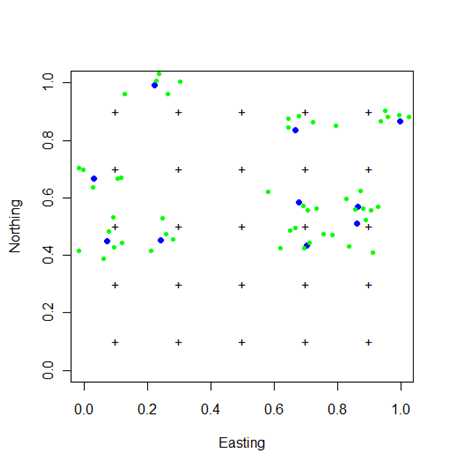
\includegraphics[height=3in]{Ch1/figs/northingeasting}
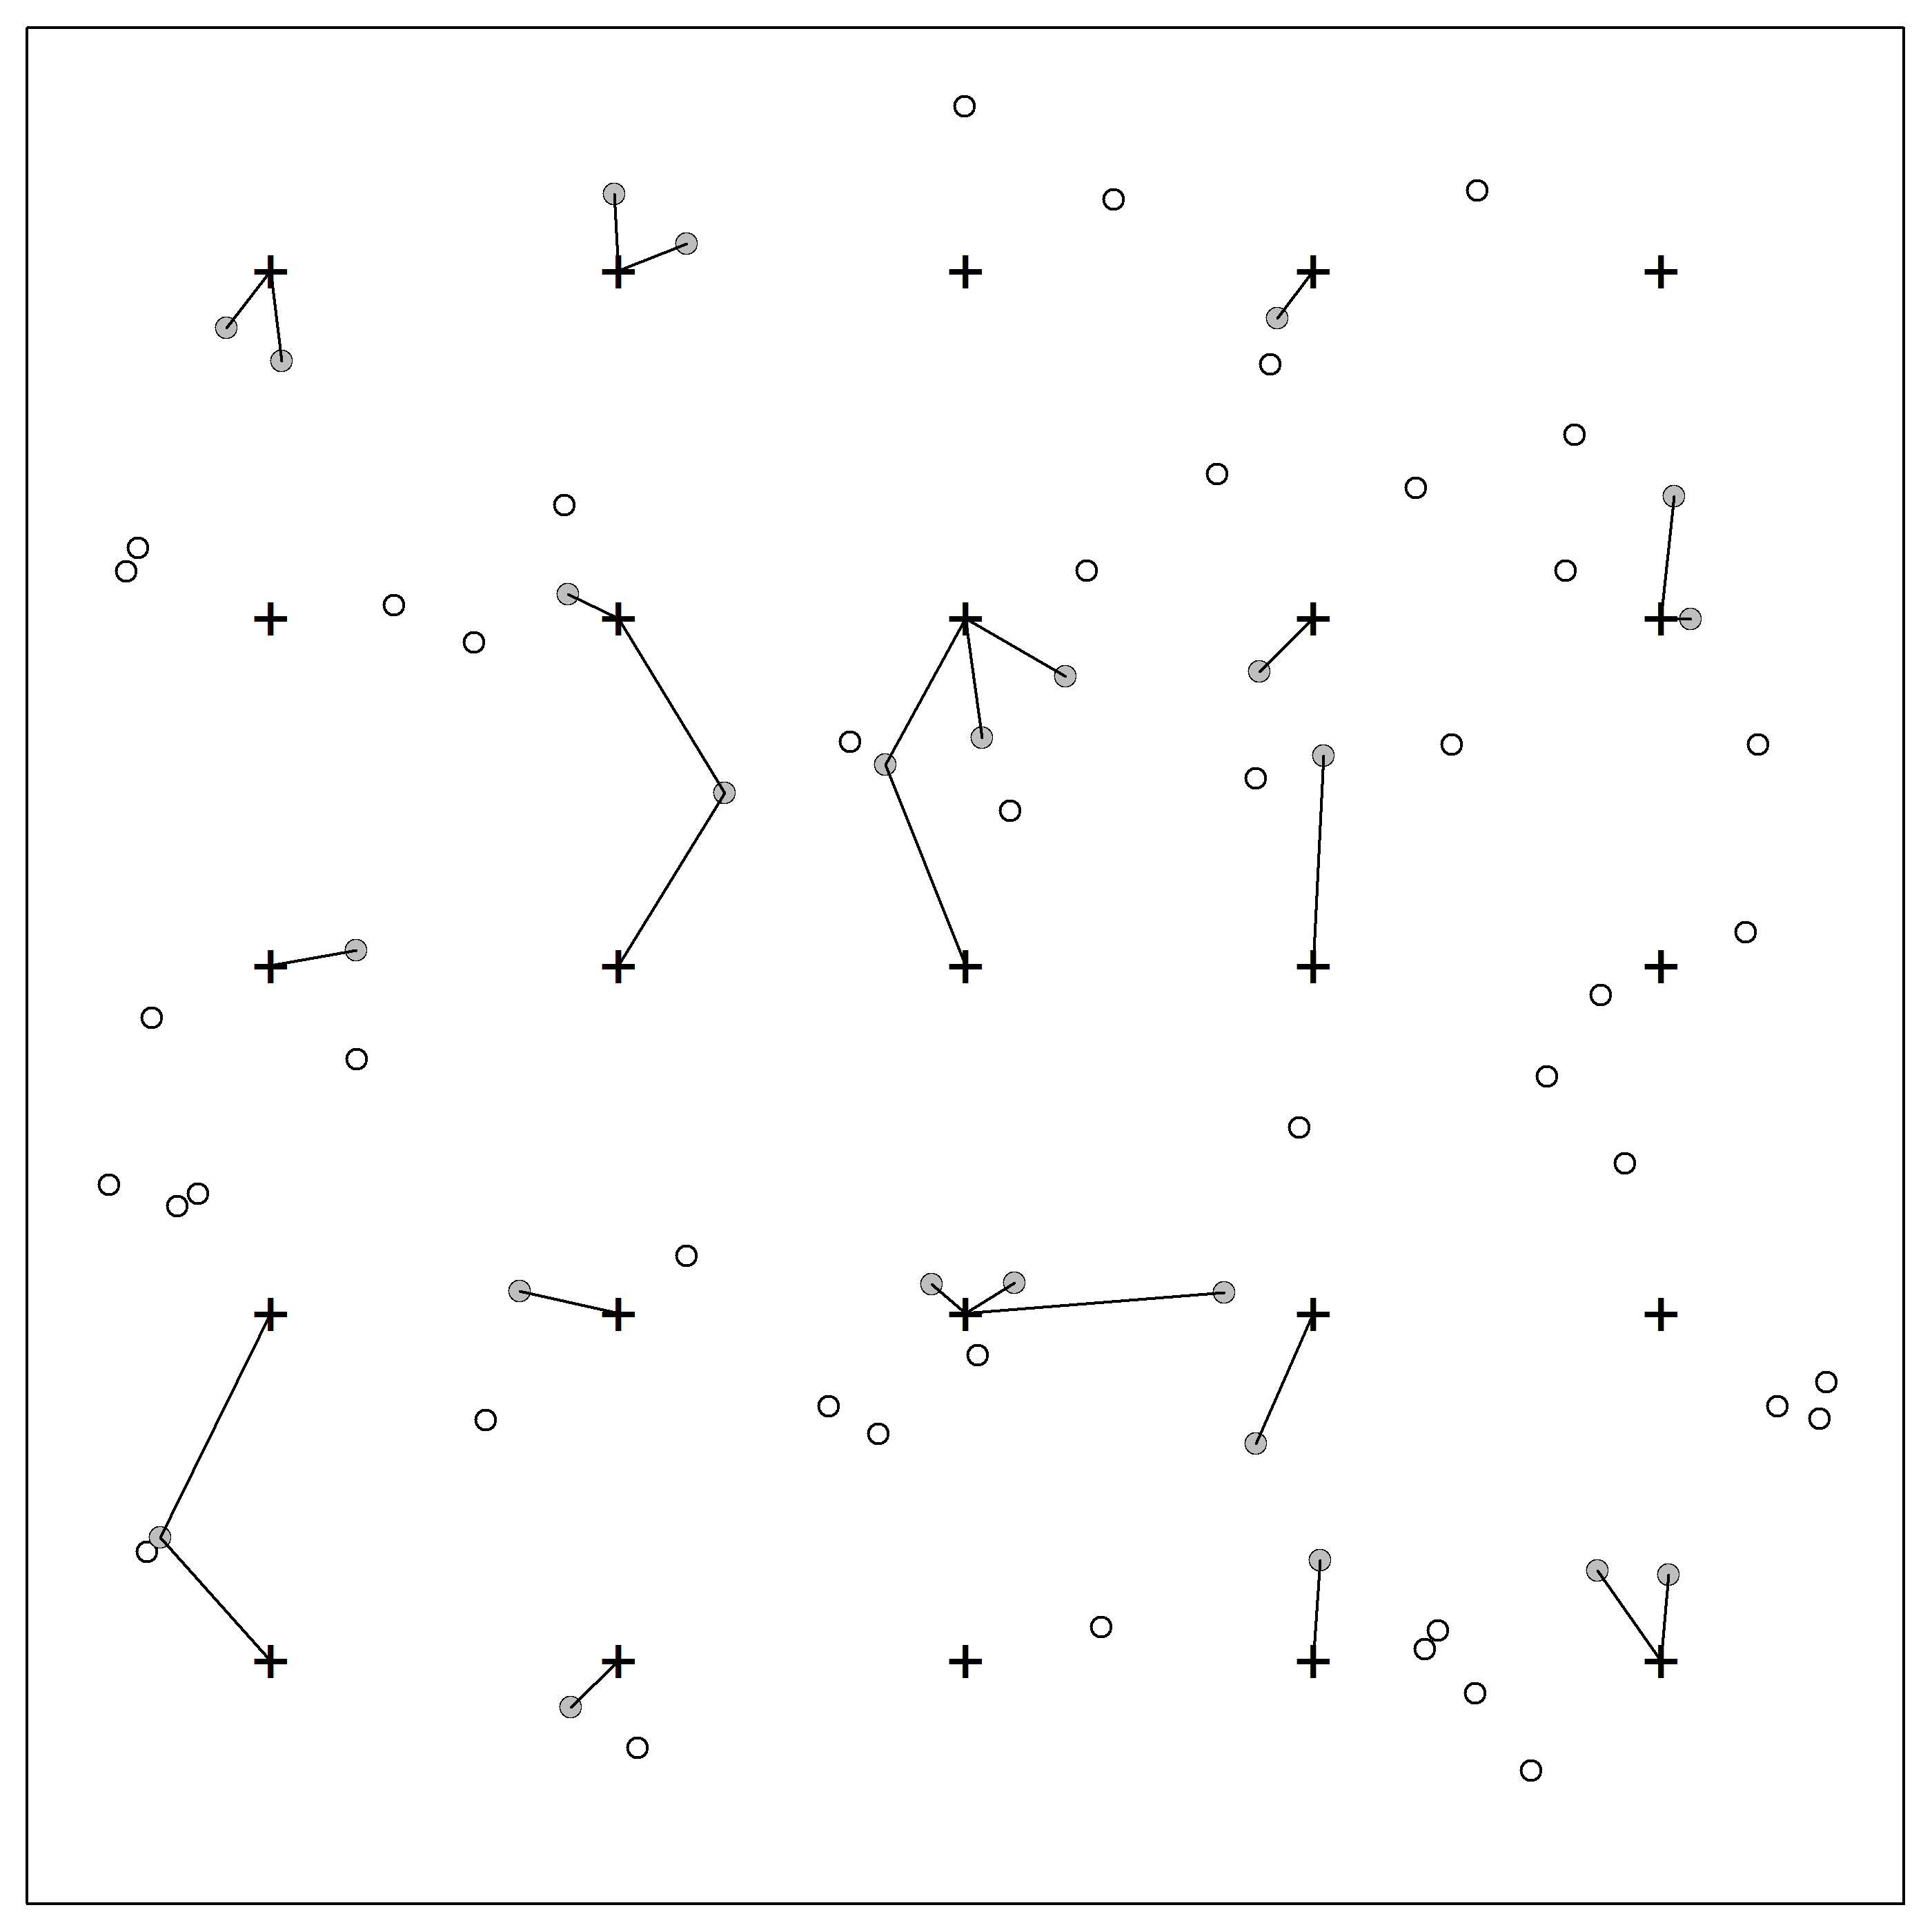
\includegraphics[width=0.5\textwidth]{Ch2/figs/SCR0}
\end{center}
\caption{Population of $N=69$ home-range centers ($\bf s$,
  circles) and 25 trap locations ($\bf x$, crosses). Lines connect
  activity centers to the traps where the individuals were
  detected. As in many SCR models, movement outcomes ($\bf u$)
  are ignored.}
\label{modeling.fig.fig1}
\end{figure}

\subsection{Variations on the SCR theme}

Having now briefly explained each of the model components in
Eq.~\ref{modeling.eq.nyus}, and having
shown how a subset of these components results in a basic SCR model,
we can now discuss other relevant arrangements.
%Although the full model including $u$ and $s$ fully describes the
%ecological process, in practice we usually work with reduced forms of
%this model.
Examples include:
(1) Classical distance sampling \citep{buckland_etal:2001, borchers_etal:2002},
(2) Spatial capture-recapture models with fixed arrays of traps
    \citep{efford:2004, borchers_efford:2008, royle_etal:2009ecol,
           royle_etal:2009jae,
           gardner_etal:2010ecol,royle_etal:2011jwm}, and
(3) Search-encounter models \citep{royle_young:2008,
  royle_etal:2011mee}. %, and
%(4) Capture-recapture distance-sampling \citep{borchers_etal:1998}.
%The constituent pieces of these models are listed in
%Table~\ref{modeling.tab.fam}.
We will now elaborate on some of these distinctions.
%of such models are:
% \begin{enumerate}
%   \item Classical distance sampling \citep{buckland_etal:2001, borchers_etal:2002}
%   \item Spatial capture-recapture models with fixed arrays of traps
%     \citep{efford:2004, borchers_efford:2008, royle_etal:2009ecol,
%            royle_etal:2009jae, gardner_etal:2010ecol,royle_etal:2011jwm}
%   \item Search-encounter models \citep{royle_young:2008, royle_etal:2011mee}.
%   \item Capture-recapture distance-sampling \citep{borchers_etal:1998}.
% \end{enumerate}
% In some classes of models, components for ${\bf u}$ and ${\bf s}$ will be confounded.
% e.g., if ${\bf s}$ are uniform in space and ${\bf u}$ is
% a random draw from some distribution centered at ${\bf s}$, then we might as
% well define ${\bf u}^{*}=\Pr({\bf u})=\int_{s} [{\bf u}|{\bf s}][{\bf
%   s}]ds$ which will itself be uniform
% for reasonable choices of $[{\bf u}|{\bf s}]$.  Some examples
% of typical spatial capture-recapture models and how
% these various model components are manifest in specific cases is
% described as follows:
\begin{enumerate}
\item {\bf Distance sampling}. The last 2 stages of the hierarchy
  are confounded (implicitly) and so analysis is based on the model
  $[y|{\bf u}*] [{\bf u}*]$. The ``process model'' is that of ``uniformity'': ${\bf u}^{*}
  \sim \text{Uniform}({\cal S})$.
%  Sometimes it is argued that distance sampling
%  estimators are ``pooling robust'' which is a way of saying they are
%  (or may be)
%  relatively insensitive to this assumption. That may be true, but the
%  construction of distance sampling estimators makes explicit the
%  uniformity assumption as a mathematical fact.

\item {\bf Spatial capture-recapture model with a fixed array of traps}.
SCR models appear to have little in common with distance sampling
because observations are made only at a pre-defined set of discrete
locations---where traps are placed. However, the models are closely
related in terms of our hierarchical representation above
%\footnote{Really
%they're kind of like point-count distance sampling where the identity
%of individuals is preserved across point samples , and distance is a
%latent variable. i.e., SCR-DS. I feel like this point should be
%emphasized somehow. Here? Later?}.
In SCR models based on fixed arrays, we cannot estimate both
$\Pr(y=1|{\bf u})$ and $\Pr({\bf u}|{\bf s})$---the probability that
an individual ``moves to ${\bf u}$'' cannot be separated from the
probability that it is detected given that it moves to ${\bf u}$,
because of the fact that the observation locations are fixed by
design.
Formally, such SCR models confound $[y|{\bf u}]$  with $[{\bf
  u}|{\bf s}]$ so that the observation model arises as:
\[
 [y|{\bf s}] = \int_{\bf u} [y|{\bf u}][{\bf u}|{\bf s}] \mathrm{d}{\bf u}
\]
This confounding happens because SCR sampling is spatially
biased---restricted to a fixed pre-determined set of locations.
Conversely,
distance sampling confounds $[{\bf u}|{\bf s}][{\bf s}]$ because, essentially, there is
only a single realization of the encounter process.
It is probably
reasonable to assume that $\Pr(y=1|{\bf u})=1$ or at least it is locally
constant for most devices (e.g., cameras, etc..), and thus the
detection model will have the interpretation in terms of movement (see
Chapt. \ref{chapt.rsf} and \ref{chapt.ecoldist}).

\item {\bf Search-encounter models}. What we call
  ``search-encounter'' models \citep{royle_young:2008,royle_etal:2011mee}
  are kind of a hybrid model combining features of SCR models and
  features of distance sampling. Like distance sampling they allow for
  encounters in continuous space which provide direct observations
  from $[{\bf u}|{\bf s}]$. Thus, the
  hierarchical model is fully identified.

  \begin{comment}
  \item {\bf Capture-recapture/distance-sampling}. See
    \citet{borchers_etal:1998}. As with the search-encounter models
    the full hierarchical model is identified: $[y|{\bf u}][{\bf
      u}|{\bf s}][{\bf s}]$ but the quantities don't really mean the
    same thing as before.

    To understand this, we expand the model to accommodate imperfect
    measurements of ${\bf u}$. Let ${\bf u}_{obs}$ be an observation
    of ${\bf u}$ (i.e., made with error). A larger hierarchical model
    is this:
    \[ [y|{\bf u}][{\bf u}_{obs}|{\bf u}][{\bf u}|{\bf s}][{\bf s}]
    \]
    If we make replicate ``instantaneous'' observations of location,
    then information is provided about $[{\bf u}_{obs}|{\bf u}]$
    (i.e., measurement error). However, in a normal distance sampling
    application, with instantaneous sampling, we don't learn anything
    about $[{\bf u}|{\bf s}]$, in effect, we are again confounding
    $[{\bf u}|{\bf s}]$ and $[{\bf s}]$: ${\bf u}^{*} = \int_{s} [{\bf
      u}|{\bf s}][{\bf s}] ds$. So the CR-DS model focuses on:
    \[ [y|{\bf u}^{*}][{\bf u}_{obs}|{\bf u}^{*}][{\bf u}^{*}].
    \]
    Structurally, this is the same basic model as the search-encounter
    model notwithstanding (1) that it is usually talked about in terms
    of repeated measures of distance instead of location and (2) the
    2nd component of the hierarchy is not movement (an ecological
    process) but rather ``measurement error'' and (3) the third
    component is not a home range center but rather a movement outcome
    (``instantaneous location'').  Thus, while the models are
    structurally identically, the meaning and interpretation of
    quantities are distinct.
  \end{comment}

\end{enumerate}


\begin{comment}
\begin{table}
  \centering
  \caption{Spatial capture-recapture models and allies.}
  \begin{tabular}{lll}
    \hline
    Description & Notation & Chapters \\
    \hline
    Full Monte            & $[n(y)|y][y|{\bf u}][{\bf u}|{\bf s}][{\bf s}]$ & --- \\
%    Distance sampling SCR hybrid & $[y|{\bf u}][{\bf u}|{\bf s}][{\bf s}]$ & --- \\
    Standard SCR         & $[y|{\bf s}][{\bf s}]$ & \ref{chapt.scr0} \\
    Distance sampling    & $[y|{\bf u}][{\bf u}]$ & --- \\
    Search-encounter SCR & $[y|{\bf u}][{\bf u}|{\bf s}]$ & \ref{chapt.search} \\
%    Mark-resight SCR     & $[n(y)|y][y|{\bf s}][{\bf s}]$ & \ref{chapt.scr-unmarked,chapt.partialID} \\
    \hline
  \end{tabular}
  \label{modeling.tab.fam}
\end{table}
\end{comment}


%These are
%mostly all semantic and conceptual distinctions which are easy to
%define in a convenient table:
%\begin{table}[ht]
%\centering
%\title{What things mean in each model.}
%\begin{tabular}{c|cc}
%           &   Search encounter models     &  CR-DS  \\  \hline
%  $\sigma$    &  movement       &   measurement error  \\
% ${\bf s}$ & activity center & instaneous location \\
%\end{tabular}
%\end{table}


\begin{comment}

\section{Analysis of spatial capture-recapture models}

\subsection{Models don't have political views!}

Whereas hierarchical modeling is a conceptual framework for
formulating models, the method of inference is independent of model
formulation. Hierarchical models can be analyzed by Bayesian and
non-Bayesian methods. A model is not Bayesian or frequentist -- what
you do to that model is Bayesian or frequentist!
\[
\bullet \mbox{"Hierarchical model"} \ne  \mbox{"Bayesian"}!!!
\]
Thus, analysis of hierarchical models is easily achieved using either
Bayesian or classical (likelihood, frequentist) methods. By
``analysis'' we mean any type of estimation, characterization of
uncertainty, prediction, model selection, or evaluation and we are not
dogmatic about our choice of inference methods. That said, we do
recognize a benefit of the Bayesian approach which is that it
emphasizes model construction and not the construction of
procedures. The Nobel prize\footnote{called something else besides
  Nobel, officially} winning econometrician Christopher Sims (Slides
from the Hotelling Lecture 6/29/2007 at Duke University - cite his
webpage) said it this way: ``Bayesian inference is a way of thinking,
not a basket of 'Methods''' Conversely, ecologistis that are subjected
to a classical statistical curriculum often have only a vague sense of
what the model is that any particular procedure is employing.  We
agree with \citet{little:2006}
that there should be more emphasis on understanding statistical
modeling, and less emphasis on statistical methods.  Toss the ``basket
of methods'' out the window and learn how to model!


We rely strictly on principles and procedures of {\it parametric
  inference} in our analysis of hierarchical models in general and,
specifically, of spatial capture-recapture models. Parametric
inference is that in which we make explicit probability assumptions
about how the data were generated. Inference procedures are then
developed under the assumption that the model is truth, because formal
parametric inference procedures that we understand the joint
probability distribution of everything that is a realization of a
random variable. {\bf There is something missing in the previous sentence. require, maybe?}There are two popular flavors of parametric
inference: {\bf Classical inference}: The joint probability distribution
of observations is the {\bf likelihood}. We maximize it to obtain MLEs
and do other fun things to it. We evaluate procedures by thinking
about what would happen over replicate realizations of data to which
our procedures are applied.  {\bf Bayesian inference} is based on the
posterior distribution, which is the joint probability distribution of
the data and also parameters and possibly other quantities including
latent variables or random effects.

Because SCR models contain a collection of latent variables - random
effects -- a natural framework for classical analysis of the models is
based on integrated likelihood \citep{laird_ware:1982,berger_etal:1999}. That is, while
the observation model is conceptualized conditional on the random
effects (the locations of individuals), classical inference is
formally based on the likelihood constructed from the {\it marginal}
probability distribution of the observations (i.e., {\it
  unconditional} on the random effect). The random effects are removed
from the conditional likelihood by integration (which is accomplished
numerically in spatial capture-recapture models). This approach to
inference has been formalized in the context of SCR models by
\citet{borchers_efford:2008, efford:2011}, and implemented for some
classes of models in the software package {\bf DENSITY} \citep{efford:2004}
and the {\bf R} package \mbox{\tt secr} \citep{efford:2011}.

Bayesian analysis is another natural framework for the analysis of
models containing latent variables or random effects.  Under this
approach, analysis of the model is based on Monte Carlo simulation
from the posterior distribution, which is the product of the
conditional likelihood, the distribution of the random effects, and
perhaps other distributions.  This approach was developed by
\citet{royle_young:2008}, and was motivated by work focused on
modeling individual effects in capture-recapture models. In
particular, a convenient reparameterization of individual covariate
models can be obtained using a method known as data augmentation
\citep{royle_etal:2007}, see \citet{royle:2008} for an application to
classical individual covariate models in \citet{royle:2008}. The close
similarity between individual covariate models and spatial
capture-recapture models, with the individual's activity center ${\bf
  s}$ being the individual covariate, led to the application of the
data augmentation method described by \citet{royle_young:2008} and subsequent papers.

These two technical formulations (classical inference based on
integrated likelihood and Bayesian inference) both provide rigorous solutions to
the inference problems posed by spatial capture-recapture data.  There
are also minor distinctions to be aware of. For example,
as a technical matter, \citet{borchers_efford:2008} and related work, assume
a Poisson point process that is unconditional on $N$ whereas Royle and
Young (2008) and related work assume a binomial point process model
which is conditional on $N$.
%More importantly, Borchers and Efford
%develop the analysis in a way that is unconditional on the point
%process (which is removed from the conditional likelihood by
%integration).  Conversely, the analysis of \citet{royle_young:2008} is
%conditional on the underlying point process. As a technical matter,
%Bayesian analysis allows us to analyze the model that is conditional
%on the underlying point process and will otherwise have more
%flexibility - open populations, using telemetry data, etc.. as will be
%demonstrated in later chapters.

We tend to favor Bayesian inference for conceptual and philosophical
reasons but we also think that  integrated likelihood
for complex point process models may prove difficult. On the other
hand, we suspect that Bayesian
analysis by MCMC
of the model that is conditional on the underlying point process will
prove to be more versatile and generalizable for complex point process
models. We say this only
tentatively and throughout this book we are not exclusive in our views
of inference and use Bayesian and classical methods of inference
interchangeable and opportunistically in this book.
We don't want to get too much into the technical foundations of
Bayesian analysis because there are many good books now including
\citet{link_barker:2010}.  \citet{kery:2010, mccarthy:2007,
  king_etal:2009} and probably others by the time this book is
finished. That said,  Bayesian analysis is introduced at a
level required to get through this book in Chapter 2.


\section{Criticisms of Hierarchical Models}

\hl{If we keep this, remove all SCR references b/c Andy will address
  those in Chapt 5}

We have frequently used the terms
``assumptions'' and ``priors'', which make some people feel
uneasy. Our view is that expressed eloquently by Link (ADD
QUOTE). Furthermore, we note that hierarchical models allow us to
modify any assumption deemed too
restrictive. That is, we can always generalize our models given enough
data. Chapter is a classic example because it addresses
perhaps the most common criticism of SCR, that ``real animals'' don't
have symmetric home ranges. In fact people have written entire papers
beating up on SCR because they \emph{assume} that this the bivariate
normal model for the encounter processes is a rigid requirement of SCR
methods. Although we believe this assumption is quite reasonable in
many contexts, Chapter \ref{chapt.ecoldist} clearly illustrates that
alternatives exist, and that SCR provides a rigorous framework for
testing for departures from this assumption, and even evaluating
hypotheses that may explain why animals move the way they do.


\end{comment}





\section{Summary and Outlook}


Spatial capture-recapture models are hierarchical models, and hierarchical
models are models of multiple random variables that are conditionally
related. It is therefore important that the basic rules of
modeling random variables are understood, and we hope that this chapter
has made some of the basic concepts accessible to ecologists with
rudimentary background in statistics. If some of this material still
seems difficult to grasp, we recommend working with the
provided \R~code, which is perhaps the best way of making the
equations more tangible.

In some respects, it is possible
to understand the jist of SCR without knowing anything about marginal
and conditional relationships. One can always fit models using canned
software and interpret the output without understanding the guts of
the model or the details of the estimation process. For some applied
ecologists, this may be perfectly fine, and this book is meant to be
useful for both statistical novices and ecologists with more advanced
quantitative skills. In most chapters, we begin with a basic conceptual
discussion, then we explain
the technical details that require an understanding of the concepts in
this chapter, and finally we end with one or more worked examples. For
those not interested in the technical details, we recommend focusing
on the chapter introductions and the examples. However, taking the
time to understand the concepts presented in this chapter can only
increase one's ability to tackle the unique and complex problems that
often present themselves when modeling spatial and temporal aspects of
population dynamics.

